\documentclass[]{article}
\usepackage[spanish]{babel}
\usepackage{graphicx}
\graphicspath{{./images/}}

\usepackage{xcolor}
\definecolor{codelistingbg}{rgb}{0.95,0.95,0.95}
\usepackage[
  cache=false,
  outputdir=/build,
]{minted}

\setminted{
    linenos=true,
    bgcolor=codelistingbg,
    fontsize=\scriptsize,
    breaklines=true
}

\usepackage[utf8]{inputenc}
\title{Omnetpy: Integración del Lenguaje Python en el Entorno de Simulación \omnetpp{}}
\author{Marcos Modenesi}


\begin{document}
\newcommand{\omnetpp}{\mbox{OMNeT++}}
\newcommand{\ui}[1]{\textit{#1}}

\maketitle
\tableofcontents

\section{Introducción}
\subsection{Objetivo}

El objetivo de esta tesis es proveer de una interfaz simple y compacta para
especificar el comportamiento de modelos de simulación para la plataforma
\omnetpp{} mediante el uso del lenguaje Python.

\subsection{Hipótesis}

Es posible definir módulos simples de \omnetpp{} en scripts escritos en Python e
integrarlos de manera que el usuario experience mínima o nula complejidad en el
proceso.

\subsection{Metodología}

La metodología en la que se basa esta tesis es extender y embeber el intérprete
de Python para que pueda recibir y transmitir comportamiento desde y hacia C++.

\subsection{Impacto}

El resultado del trabajo (disponible en https://github.com/mmodenesi/omnetpy/)
resulta beneficioso para personas que buscan aprovechar la plataforma \omnetpp{}
para realizar simulaciones, pero para quienes la programación directa en C++
resulta un obstáculo. En particular, facilita la utilización de \omnetpp{} como
herramienta pedagógica en cursos de ciencias de computación donde los
estudiantes suelen contar con un dominio bastante bueno de Python, pero en
general desconocen C++.  El interés de este proyecto ha sido reconocido por los
desarrolladores de \omnetpp{} (https://omnetpp.org/download-items/omnetpy.html).

\subsection{Estructura}

El capítulo~\ref{sec:eda} de esta tesis presenta el estado del arte alrededor
de \omnetpp{} y la simulación de eventos discretos. Se realiza una comparación
entre C++ y Python. El capítulo~\ref{sec:met} presenta la metodología. El
capítulo~\ref{sec:des} discute el detalle del desarrollo. La herramienta
omnetpy se presenta en el capítulo~\ref{sec:omnetpy}. El capítulo~\ref{sec:ev}
evalúa cualitativa y cuantitativamente omnetpy. Las conclusiones se resumen en
el capítulo~\ref{sec:conc}, así como los desafíos abiertos.

\section{Estado del arte}\label{sec:eda}

\subsection{Simuladores de eventos discretos}

Un sistema es una colección de entidades que interactúan bajo ciertas reglas
para alcanzar un fin común. Decimos que un sistema es \textit{continuo} cuando
las variables que permiten describir su estado cambian de forma contínua con
respecto al tiempo (por ejemplo, altura y velocidad de un avión). En oposición,
los sistemas \textit{discretos} son aquellos en los que las variables de estado
cambian de forma instantánea en determinados momentos en el tiempo (por
ejemplo, cantidad de clientes en una estación de servicio).

A menudo es de interés estudiar un sistema para entender los parámetros que
gobiernan su funcionamiento, realizar mejoras o comprender de qué manera serán
impactados por ciertos cambios en sus entradas.

Para llevar a cabo un estudio de esta naturaleza, una primera opción es
experimentar con el sistema real. No obstante, esto no siempre es deseable
(podría implicar muchos gastos y disrupciones en el funcionamiento normal del
sistema) o siquiera posible (quizás el sistema aún no ha sido construido).
Entonces se puede recurrir a experimentar con un \textit{modelo} del sistema.

Un modelo puede ser \textit{físico} (modelo a escala) o \textit{matemático}.
Este último consiste en una serie de suposiciones sobre el funcionamiento del
sistema que se pueden formalizar en un conjunto de relaciones matemáticas y
lógicas entre las entidades que lo componen.

A veces un sistema es lo suficientemente sencillo como para que el modelo
matemático del mismo pueda ser resuelto analíticamente, mediante el uso de
herramientas tales como el cálculo diferencial, álgebra, teoría de
probabilidad. Sin embargo, cualquier modelo más o menos interesante de un
sistema no trivial suele ser muy complejo para ser tratado mediante estos
métodos. Aparece entonces la simulación como una forma de ganar comprensión
sobre el funcionamiento del sistema.

\begin{figure}[h]
\caption{Formas de estudiar un sistema}
\centering
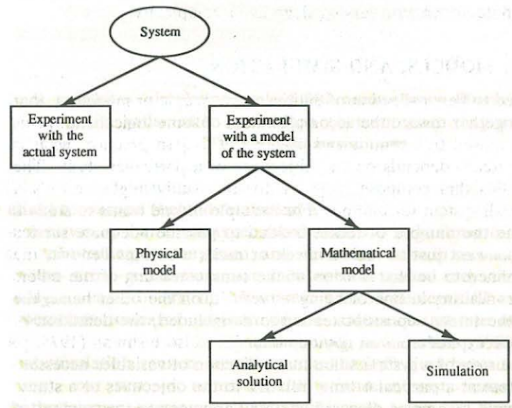
\includegraphics[width=8cm]{taxonomia_enfoques}
\end{figure}

En una simulación, el modelo no es resuelto, sino que es \textit{ejercitado}
con el fin de recolectar información a partir de la cual se puedan realizar
estimaciones sobre los valores de los parámetros de interés.

En los modelos estáticos no es relevante el paso del tiempo. Un ejemplo de
simulación de este tipo lo ofrece el método Monte Carlo. En los modelos
dinámicos, en cambio, el tiempo es relevante ya que se estudia la evolución del
sistema a través de una línea temporal artificial.

La construcción de una simulación ofrece las siguientes ventajas:
\begin{itemize}
    \item Nuevas políticas, procedimientos de operación, reglas de decisión,
flujos de información, procedimientos de organización, etc. pueden ser
explorados sin perturbar la operación del sistema real.

    \item Nuevos diseños pueden ser probados sin asignar recursos a la
adquisición de elementos físicos, antes de implementar cambios en el mundo
real.

    \item Permite validar hipótesis y responder a preguntas de tipo ``¿qué
pasaría si...?''.

    \item El diseño de la simulación permite ganar conocimiento sobre el
sistema bajo investigación.

    \item Permite cambiar los valores de entrada para observar cambios en las
salidas, lo cual facilita una mayor comprensión sobre cuáles son las variables
más relevantes y cómo interactúan.

    \item Proporciona una herramienta de gran valor pedagógico.

    \item Permite verificar soluciones analíticas.

    \item El tiempo es artificial, y por lo tanto puede ser contraído (simular
meses o años de funcionamiento de un sistema en algunos minutos), expandido
(observar cambios que de otra forma serían demasiado rápidos) e incluso pausado
y avanzado manualmente.

    \item El concepto básico de una simulación es fácil de interpretar, por lo
tanto puede ser una herramienta útil a la hora de justificar decisiones a
clientes, inversores, gestores, etc.

    \item Puede ser más creíble que un modelo matemático resuelto de forma
analítica, porque necesita hacer menos simplificaciones.
\end{itemize}

La simulación de eventos discretos involucra el modelado de un sistema y su
evolución mediante una representación en la cual las variables de estado
cambian de forma instantánea en determinados puntos del tiempo. Estos puntos
del tiempo son aquellos en los que un evento ocurre, donde un evento está
definido como una ocurrencia instantánea que tiene la potencialidad de cambiar
el estado del sistema. Decimos que hay una potencialidad de cambiar el estado
del sistema porque un evento puede utilizarse de manera que no cambie el
sistema pero que cumpla otros fines. Por ejemplo, se puede programar un evento
que dará fin a la simulación en un tiempo particular.

Si bien en principio sería posible llevar a cabo una simulación de eventos
discretos a mano, registrando el estado del modelo ante cada nuevo evento, la
cantidad de información que habría que manipular para simular cualquier sistema
del mundo real hace que esta tarea sólo sea abordada mediante el uso de
software especializado.

Un simulador de eventos discretos es un programa destinado a soportar la
simulación de sistemas mediante modelos dinámicos y discretos. En dichos
programas es común encontrar los siguientes componentes:

\begin{itemize}
    \item Estado del sistema: colección de variables necesarias para describir
el sistema en un punto particular del tiempo.

    \item Reloj de simulación: una variable especial para llevar cuenta del
tiempo.

    \item Lista de eventos: una lista con los eventos futuros.

    \item Contadores: variables usadas para almacenar información estadística
sobre el desempeño del sistema.

    \item Fuentes de variables aleatorias para las distribuciones más comunes.

    \item Herramientas de recolección y manipulación de datos, procesamiento
estadístico y representación visual de los mismos.

    \item Interfaz gráfica que proporciona una representación visual del
sistema (en dos o tres dimensiones), mostrando animaciones que ayudan al
seguimiento de los cambios de estado.
\end{itemize}

Las fuentes consultadas en la confección de este capítulo fueron [1], [2], [3].

\subsection{Simulador \omnetpp{}}

Objective Modular Network Testbed in C++ (\omnetpp{}) es un simulador de eventos
discretos modular y orientado a objetos, escrito en el lenguaje de propósito
general C++. Originado en 1997 por András Varga, es un software de código
abierto que puede ser utilizado libremente para usos no comerciales
(principalmente investigación y enseñanza). Existe una extensión de \omnetpp{}
para usos comerciales llamada OMNEST.

Principalmente orientado a la simulación de sistemas de comunicación,
multiprocesadores y otros sistemas distribuidos, \omnetpp{} es lo suficientemente
general como para resultar de utilidad en otros dominios (diseño de protocolos,
validación de arquitecturas de hardware, evaluación de desempeño de sistemas de
software, y en general, cualquier sistema donde el enfoque de eventos discretos
sea apropiado y pueda ser convenientemente mapeado a un conjunto de entidades
que intercambian mensajes).

Su diseño modular hace posible que ciertas piezas centrales de la simulación de
redes que no son parte del paquete principal (por ejemplo, librerías de
simulación de protocolos TCP) aparezcan espontáneamente desde una comunidad de
usuarios muy activa.

\omnetpp{} hace mucho énfasis en la facilidad de depuración y trazabilidad de
los elementos constituyentes del modelo, para lo cual es posible ejecutar las
simulaciones en un ambiente de interfaz gráfica que presenta animaciones para
los eventos (mensajes) y brinda facilidad de inspección de los módulos
intervinientes.

También es posible ejecutar simulaciones en un ambiente de consola (es decir,
sin interfaz gráfica), útil para la ejecución en lote de varios experimentos.

Ofrece soporte para simulaciones de gran escala preparadas para ser
paralelizadas en un cluster de computadoras.

Busca apoyarse en interfaces abiertas (archivos de texto plano, formatos
comunes) para posibilitar la interacción con otras herramientas.

\subsubsection{Introducción a \omnetpp{}}

En esta sección se describen en detalles los diferentes componentes de un
modelo de simulación de \omnetpp{} desde la perspectiva del usuario.

\paragraph{Modelos y estructura jerárquica}

En \omnetpp{}, un modelo consiste de módulos que se comunican mediante el paso de
mensajes. Los módulos simples se escriben en el lenguaje de programación C++,
utilizando clases de la librería de simulación. Estos módulos simples
constituyen el componente atómico (no se pueden subdividir) y activo (es donde
el usuario introduce la lógica del modelo) del modelo.

Estableciendo una estructura jerárquica sin límite de niveles, los módulos
simples pueden ser agrupados en módulos compuestos, lo cual permite dividir los
modelos complejos en partes más pequeñas, o agrupar varias partes en un único
módulo. Esta es una decisión de diseño que corre por cuenta del usuario. 

Los módulos se comunican mediante el paso de mensajes. Además de una marca de
tiempo, los mensajes pueden tener cualquier tipo de atributo. Los módulos
presentan compuertas de entrada y de salida que constituyen su interfaz.  Los
mensajes usualmente se destinan a compuertas, pero también es posible enviarlos
directamente a módulos específicos.

Los módulos pueden tomar parámetros, utilizados para pasar configuraciones y
definir la topología del sistema. Asimismo, las conexiones entre módulos pueden
tener atributos (demora de propagación, tasa de error, tasa de transferencia),
permitiendo definir conexiones como tipos (canales) para reutilizarlos.

Los parámetros pueden tomar valores específicos, declarados en archivos de
configuración, o pueden ser tomados de una fuente de valores aleatorios. 

\paragraph{El lenguaje NED}

NED es un lenguaje declarativo creado específicamente para \omnetpp{}, en el cual
el usuario define la estructura del modelo (módulos e interconexiones).

Una definición de modelo puede constar de declaraciones de módulos simples,
módulos compuestos y definiciones de la red:

\begin{itemize}
    \item Los módulos simples describen su interfaz: compuertas y parámetros.

    \item Los módulos compuestos son definidos mediante la declaración de su
interfaz externa (compuertas y parámetros) así como la definición de sus
submódulos y sus interconexiones.

    \item La definición de una red típicamente define al modelo como una
instancia de un módulo particular.
\end{itemize}

Las definiciones NED soportan la partición en diferentes archivos mediante el
mecanismo de inclusión.

\omnetpp{} incluye un editor gráfico que toma como partida los archivos NED. El
usuario puede hacer cambios tanto en la vista gráfica como directamente en el
texto del archivo, y cambiar de vista en cualquier momento.

NED es un lenguaje declarativo que contiene constructos parecidos a los
condicionales y los bucles de un lenguaje imperativo, lo que posibilita
parametrizar las topologías. Esto es una ventaja sobre otros simuladores donde
o bien no es posible parametrizar (sólo se pueden expresar topologías fijas) o
donde la especificación del modelo se mezcla con la lógica de la simulación,
haciendo imposible la edición gráfica.

El lenguaje NED es compatible con el formato XML, lo que posibilita la carga
dinámica de modelos que provengan de otras fuentes.

\paragraph{Programación de módulos simples}

Los módulos simples son los elementos activos del sistema y funcionan como
bloques constituyentes de los módulos complejos y, en última instancia, del
modelo de simulación.

El usuario implementa la funcionalidad de un módulo simple heredando de la
clase \verb!cSimpleModule!, que es parte de las librerías de simulación de
\omnetpp{} y puede optar por dos paradigmas de programación diferentes:

\begin{itemize}
    \item basado en corrutinas
    \item basado en el procesamiento de eventos
\end{itemize}

En el paradigma basado en corrutinas, el código del modelo corre en su propio
hilo, el cual recibe el control del kernel cada vez que el módulo recibe un
mensaje. Típicamente, este código nunca incluye un \verb!return!: sus puntos de
entrada son llamadas a \verb!receive! (esperar el siguiente mensaje) y sus
puntos de salida son llamadas a \verb!send! (enviar un mensaje)

En el paradigma basado en el procesamiento de eventos, el kernel de simulación
llama a una función específica del módulo (\verb!handleMessage!) con el mensaje
como argumento. Esta función debe ejecutar un \verb!return! al terminar de
procesar el mensaje, efectivamente devolviendo el control al kernel de
simulación.

Además de el código destinado al envío y recepción de mensajes, es posible
escribir código que se ejecuta durante la inicialización y finalización del
módulo (este último, sólo si la simulación terminó exitosamente).

Como parte de la simulación, un módulo puede cambiar sus entradas y salidas, o
crear dinámicamente nuevos módulos, lo cual hace posible modificar la topología
inicial de la red.

\paragraph{Separación del modelo y los experimentos}

Como se describió anteriormente, el comportamiento del modelo es capturado en
archivos C++ mientras que la topología es capturada en archivos NED.

En una simulación cualquiera, uno está generalmente interesado en conocer cómo
se comporta el modelo a partir de diferentes datos de entrada. Esta información
no pertenece ni a los archivos C++ ni a los archivos NED: la configuración de
los experimentos se coloca en otros archivos, con extensión \verb!ini!. En
ellos se puede especificar cuántas corridas de una simulación se desea
realizar, con qué valores para los parámetros, con qué distribuciones
aleatorias, cuánto tiempo puede durar como máximo la simulación, etc.

\paragraph{Entorno de desarrollo integrado}

La edición de los diferentes archivos que intervienen (archivos de C++,
archivos NED, archivos ini) puede realizarse cómodamente desde un Entorno de
Desarrollo Integrado (IDE, por sus siglas en inglés) que es parte de la
distribución oficial de \omnetpp{}. Las ventajas de programar desde este IDE son
múltiples:

\begin{itemize}
    \item Introspección de código, navegación a la definición de una variable,
navegación a la documentación.

    \item Asistencia para operaciones comunes de refactorización de código.

    \item Acceso rápido a funcionalidades comunes como compilación o ejecución.

    \item Resaltado de sintaxis de los diferentes lenguajes

    \item Depuración de código.

    \item Asistente para la generación de nuevos proyectos.

    \item Edición de archivos NED desde la vista gráfica.
\end{itemize}

A su vez, este entorno de desarrollo integrado ofrece la posibilidad de
visualizar gráficos de diversos tipos a partir de los datos generados durante
una simulación.

\paragraph{Ejecución de una simulación}

El código de los módulos simples se compila enlazando con las librerías de
simulación de \omnetpp{} creando un binario que constituye el ejecutable de la
simulación. Cambios posteriores a los archivos NED (cambios en la topología y
en los parámetros) o en los archivos \verb!ini! (cantidad y duración de las
simulaciones, distribuciones de las variables aleatorias, valores de los
parámetros) no requieren nuevos pasos de compilación.

El binario de la simulación puede ejecutarse de forma que la misma se
corra en un entorno gráfico apto para la visualización y depuración del modelo,
o sin este entorno gráfico (más apropiado para correr muchas simulaciones en
lote).

\subsubsection{Ecosistema y casos de uso}

Desde sus comienzos, cerca del año 2000, \omnetpp{} ha tenido una amplia recepción
en entornos de investigación, educativos, así como también en la industria.
Diversos proyectos independientes han aportado nuevas librerías reutilizables y
modelos de dominios específicos, algunos de los cuales se listan a
continuación:

\begin{itemize}
    \item INET Framework [7] provee soporte para simulaciones de redes de
comunicación que utilizan los protocolos de Internet (TCP, UDP, IPv4, IPv6,
OSPF, BGP, etc.), así como protocolos cableados e inalámbricos de la capa de
enlace (Ethernet, PPP, IEEE 802.11, etc.) y soporte para redes móviles,
protocolos MANET (Mobile Ad Hoc Networks), DiffServ, etc. Muchos otros
proyectos toman INET como base y la extienden en direcciones específicas, como
redes de vehículos, overlay, P2P, LTE.

    \item Simu5G [8][9] producto de un proyecto de investigación conjunta entre
Intel Corporation y el Computer Networking Group de la Universidad de Pisa,
Italia, provee soporte para redes 5G NewRado.

    \item SimulLTE [10][11] provee librerías para la simulación de redes LTE y
LTA.

    \item Veins [12][13] es un framework de simulación de código abierto de IVC
(Inter-Vehicular Communication) que utiliza \omnetpp{} para la simulación de
redes así como SUMO, un simulador de tráfico vehicular, usando cosimulación.

    \item CoRE4INET[14] es una extensión a la herramienta INET para
simulaciones basadas en eventos de real-time Ethernet dentro del simulador
\omnetpp{}.

\end{itemize}

Una lista completa puede conseguirse visitando el sitio de \omnetpp{} [16].

Desde el año 2008 en forma continuada, la comunidad de \omnetpp{} se reúne
anualmente en un evento en el que se comparten experiencias, casos de usos y se
realizan ``hackatones'', maratones de programación en los que se busca atacar
un problema concreto de forma creativa en pocas horas. Algunos de los temas
presentados:

\begin{itemize}
    \item Development and Testing of Automotive Ethernet-Networks together in
one Tool - \omnetpp{} (Patrick Wunner, Stefan May, Kristian Trenkel, and
Sebastian Dengler)

    \item Implementation of an Adaptive Energy-efficient MAC Protocol in
\omnetpp{} / MiXiM (Van Thiep Nguyen, Matthieu Gautier, and Olivier Berder)

    \item Attack of the Ants: Studying Ant Routing Algorithms in Simulation and
Wireless Testbeds (Michael Frey and Mesut Günes)

    \item Modeling Quantum Optical Components, Pulses and Fiber Channels Using
\omnetpp{} (Ryan D. L. Engle, Douglas D. Hodson, Michael R. Grimaila, Logan O.
Mailloux, Colin V. McLaughlin and Gerald Baumgartner)

    \item High Frequency Radio Network Simulation Using \omnetpp{} (Jeffery
Weston and Eric Koski)

    \item Stacked-VLAN-Based Modeling of Hybrid ISP Traffic Control Schemes and
Service Plans Exploiting Excess Bandwidth in Shared Access Networks (Kyeong Soo
Kim)

    \item DoS Protection through Credit Based Metering - Simulation Based
Evaluation for Time-Sensitive Networking in Cars (Philipp Meyer, Timo Häckel,
Franz Korf and Thomas Schmidt).
\end{itemize}

Para una lista completa se recomienda visitar la página oficial de los archivos
de la conferencia. [17].

Las fuentes consultadas en la confección de este capítulo fueron [4], [5], [6]

\subsection{Otras herramientas similares}

Esta sección presenta brevemente los principales proyectos que cumplen el rol
de simulador de eventos discretos, sus características y sus diferencias con
\omnetpp{}. En particular, se toma el caso de SimPy que es, hasta donde alcanza
nuestro conocimiento, el único programa de este tipo basado en el lenguaje
Python.

\subsubsection{ns3}

Herramienta orientada a la simulación de redes de comunicación, dirigido
principalmente al uso académico y educativo [18]. Es un proyecto de código
abierto, gratuito, liberado bajo la licencia GNU GPLv2 mantenido por su
comunidad. Está basado en C++ y parte de la API de simulación cuenta con
``bindings'' (enlaces) para Python que son generados automáticamente (hasta
donde este proceso es automatizable) y cuya completitud y correctitud no es el
principal objetivo del proyecto [19].

A diferencia de \omnetpp{}, la simulación y la visualización (depuración,
trazabilidad) son temas separados. Por defecto, no presenta interfaz gráfica
para mostrar animaciones de los modelos. Las trazas generadas durante una
simulación pueden procesarse en otro software denominado NetAsim que permite la
visualización, o incluso en otros programas no relacionados, como WireShark.
Existe también una extensión (PyViz) que permite realizar una visualización
interactiva (es decir, durante la simulación) pensada con propósitos de
depuración.

A pesar de su filosofía de modularización, esta herramienta no separa los
múltiples aspectos de una simulación (lógica, configuración, topología) en
diferentes archivos, si no que todo esto se realiza directamente mediante el
código C++. Por esta razón, el usuario tiene que proveer más código C++ que en
una simulación típica de \omnetpp{}, ya que el programa incluye desde el
tratamiento de los argumentos del programa (si los hubiere), la declaración y
configuración de los nodos, los canales, las aplicaciones, el nivel de logging,
etc, hasta la misma inicialización y finalización de la simulación.

Es una herramienta que supone que el usuario está muy familiarizado con el
entorno de línea de comandos y puede configurar y compilar sus fuentes con
facilidad para producir el binario adaptado a sus necesidades.

\subsubsection{NetSim}

NetSim parece ser un nombre bastante común para este tipo de software. En
particular, aquí hablamos de la herramienta producida por la compañía india
Tetcos [20]. NetSim v1 apareció en 2005 y se encuentra actualmente en la
versión 13 (mayo 2021).

Esta herramienta, escrita en lenguaje C, corre sobre plataformas Windows y se
distribuye bajo diferentes licencias comerciales. Existe incluso una licencia
especial para usos académicos y educativos, que también es paga.

Está orientada a la simulación de redes de comunicación, para lo cual provee
una extensa librería con los protocolos y elementos necesarios (de acuerdo al
tipo de licencia obtenida).

El principal caso de uso es el de establecer un escenario de simulación
ubicando componentes (nodos, aplicaciones, enlaces) en una grilla espacial, y
caracterizando los canales de comunicación, para luego correr la simulación y
recoger métricas que permitan sacar conclusiones.

El usuario sólo puede implementar sus propios algoritmos o recolectores de
datos editando el código fuente de NetSim y volviendo a compilar.

\subsubsection{SimPy}

Se trata de una librería de código abierto para escribir simulaciones de
eventos discretos en lenguaje Python, distribuida bajo una licencia MIT que
posibilita su uso libre [21].

La simulación se estructura alrededor del concepto de \textit{proceso}, que
constituye el elemento activo de la simulación (un cliente, un coche, un nodo
de una red), haciendo uso de generadores.

Los procesos se programan utilizando generadores.  En Python, un generador es
un tipo especial de función que incluye la palabra reservada \verb!yield!. Al
ejecutar la instrucción \verb!yield!, la función es pausada y el control
retorna al código que la llamó. Posteriormente, la ejecución de la corrutina se
puede reanudar, desde el mismo punto donde cedió el control. Esta
característica del lenguaje Python ofrece un recurso que SimPy utiliza para
estructurar la simulación, en un modelo de corrutinas (funciones que ceden el
control voluntariamente en lo que se denomina concurrencia cooperativa).

Estos generadores crean eventos y ceden el control al orquestador de la
simulación cuando ejecutan un \verb!yield!. Cuando el evento \textit{ocurre}
(llega su momento en el tiempo de la simulación) el proceso continúa.

Simpy incluye también funcionalidad para modelar el uso de recursos
compartidos y la interacción de procesos.

Es importante notar que SimPy es simplemente una librería que implementa el
código básico para estructurar una simulación, pero no provee muchas de las
funcionalidades que las otras herramientas tienen incorporadas (interfaz
gráfica, animación, recolección de datos, configuración de experimentos,
visualización de resultados, etc.).

\subsection{C++ vs. Python}

Analizando herramientas de simulación de eventos discretos, lo más común es
encontrar que se ha utilizado un lenguaje de bajo nivel como C o C++, siendo
SimPy, hecho en Python, un caso excepcional. En esta sección se hace una breve
comparación entre C++ y Python, para entender qué se gana y qué se pierde al
utilizar cada lenguaje. Esto nos permitirá fundamentar mejor por qué este
proyecto toma la iniciativa de permitir la utilización de la herramienta
\omnetpp{} (escrita en C++) desde código escrito enteramente en Python.

\subsubsection{Generalidades}

Originado por Bjarne Stroustrup en 1979 como una extensión del lenguaje C que
añadía soporte para programación orientada a objetos, C++ fue concebido para la
programación de sistemas operativos y sistemas embebidos, así como para
software con recursos escasos, con metas tales como performance y eficiencia.
Ha sido utilizado en muchos otros contextos [22], como ser aplicaciones de
escritorio, videojuegos, servidores, y también en aplicaciones de alta
criticidad (enlaces telefónicos o sondas espaciales).

Se trata de un lenguaje compilado, por lo que se puede utilizar en cualquier
plataforma para la cual exista un compilador de C++.

En el año 1998, el lenguaje fue estandarizado por la International
Standarization Organization (ISO). A dicho estándar siguieron ampliaciones y
modificaciones en los años 2003, 2011, 2014, 2017, siendo el último estándar
publicado en 2020 en lo que se denomina informalmente C++20.

Python fue originado a finales de la década de 1980 por Guido Van Rossum, y
conoció su primera edición oficial en 1991. La versión más reciente del
lenguaje, al momento de escribir este documento, es la 3.10, liberada en
octubre de 2021. Desde sus inicios, el lenguaje ha puesto énfasis en producir
un lenguaje fácil de escribir y de leer, poniendo el acento en que el tiempo de
las personas es más valioso que el tiempo del CPU.

El desarrollo y crecimiento del lenguaje es guiado por una organización sin
fines de lucro llamada Python Software Foundation [25].

\subsubsection{Sintaxis}

C++ hereda su sintaxis del lenguaje C, terminando cada sentencia con punto y
coma y delimitando bloques por medio de corchetes. 

En general, Python tiene una sintaxis más sencilla, con menos palabras clave y
utiliza sangrías para definir bloques de código. Leer un programa en Python
muchas veces se puede asemejar a leer un texto en inglés.

\subsubsection{Forma de uso}

C++ es un lenguaje compilado. El código fuente es finalmente convertido a un
formato binario que puede ser ejecutado instrucción por instrucción por el
procesador de la computadora. Un paso intermedio realizado por una herramienta
conocida como ``preprocesador'' puede además realizar cambios en el conjunto de
caracteres escrito directamente por el programador, insertando otros archivos
(directiva \verb!#include!), incluyendo o excluyendo ciertos bloques (directiva
\verb!#ifdef!) o también expandiendo lo que comúnmente se conoce como ``macros''.
Esto agrega un nivel de dificultad más a la sintaxis de C++, ya que lo que el
programador escribe, no suele ser exactamente igual a lo que el compilador
recibe para convertir a binario.

Python no es un lenguaje compilado, como C++, C o go, si no que es un lenguaje
interpretado: el código fuente no es convertido directamente a código máquina
para su ejecución en un procesador. El código escrito en Python debe ser
proporcionado a un programa especial que se conoce como ``intérprete''. Tras
una primera etapa de preprocesado (parseo, elaboración del AST, generación de
bytecode propio de Python), el intérprete se encarga de llevar adelante la
ejecución instrucción por instrucción. Este intérprete es en sí mismo un
programa que se llama comúnmente ``Python'' (o también Python3, Python35,
etc., dependiendo de la versión).

No existe un único intérprete de Python. El más popular y difundido, conocido
como ``cPython'', es el intérprete de referencia de Guido Van Rossum (creador
del lenguaje) escrito en C. Puede considerarse la implementación oficial: se lo
referencia como ``Python'' y se usa el término ``cPython'' (como en este
párrafo) cuando se busca distinguirlo de otras implementaciones [23].

Notar que el término ``Python'' tiene (al menos) dos significados:

\begin{itemize}
    \item Es un lenguaje de programación definido mediante ciertas reglas
sintácticas que delimitan las cadenas de caracteres que constituyen un programa
válido y las separan de aquellas que, contrariamente, no son programas válidos
[24].

    \item Es un binario que sirve de intérprete (ejecutor) de ciertos programas
escritos usando tales reglas sintácticas.
\end{itemize}

A lo largo de este trabajo, cuando hablamos de ``Python'' nos referimos al
lenguaje. Para referirnos al binario que ejecuta archivos fuente en este
lenguaje, hablamos del ``intérprete'' o ``intérprete de Python''. Más
específicamente, nos referimos a la implementación oficial en C (cPython). 

\subsubsection{Distancia al hardware}

El factor que hace que un lenguaje sea considerado de alto o bajo nivel es su
distancia a los detalles físicos de la computadora que ejecuta el código.
En el nivel más bajo posible, podríamos intentar escribir un programa
cuidadosamente disponiendo ceros y unos de forma de componer un archivo binario
que llegara a ser ejecutable por el procesador. Un poco por encima de este
nivel, podríamos utilizar lenguaje assembly. Si bien aquí no se utilizan ceros
y unos directamente, sí se manipulan los registros del microprocesador, se
direcciona la memoria manualmente, se opera al nivel de bytes.

En general, en lenguajes de tan bajo nivel, se gana un control extremo sobre el
uso del hardware, pero se invierte un tiempo enorme en realizar tareas
triviales, y se hace en extremo difícil evitar errores.

Si bien C++ presenta muchas características de lenguaje de alto nivel, en
general no hay una gran abstracción sobre los detalles de una computadora. Por
el contrario, el lenguaje brinda herramientas para aprovechar esos detalles.
Como ejemplo, pensemos que quien programa tiene a su disposición diversos tipos
de datos para representar un entero (\verb!char!, \verb!int!, \verb!short int!,
\verb!long int!, \verb!long long int!, en sus versiones \verb!signed! o
\verb!unsigned!) lo cual permite elegir el más apropiado para cada aplicación
(según el rango de valores que se necesite representar, y la cantidad de
memoria que se pueda invertir en ello), pero también agrega un nivel de
dificultad extra para quien no domina los detalles. Python es considerado un
lenguaje de alto nivel. No busca exponer los detalles internos de la máquina
virtual ni de la máquina física subyacente. Esto, por supuesto, puede venir con
una penalidad en la performance y una ganancia en la usabilidad del lenguaje.

\subsubsection{Paradigmas soportados}

C++ es un lenguaje imperativo que puede utilizarse principalmente para escribir
programas de paradigma procedimental u orientado a objetos. Asimismo, una
característica del lenguaje que son los llamados templates o ``plantillas''
habilita a formas de programación genérica (código genérico cuya información de
tipo será definida en tiempo de compilación).

Python también es un lenguaje imperativo y soporta fuertemente los paradigmas
procedimental y orientado a objetos. Si bien no es un lenguaje funcional,
incluye características que permiten la adopción de un estilo de programación
funcional. Soporta también la programación orientada a aspectos y
metaprogramación.

\subsubsection{Sistema de tipos}

C++ emplea un sistema de tipos estático (toda variable tiene un tipo),
explícito (el tipo de la variable debe ser declarado, es parte del código
fuente). Como el tipo de cada variable se conoce en tiempo de compilación,
muchos errores de tipado son detectados y prevenidos por el compilador.

Python, en cambio, emplea un sistema de tipos dinámico, implícito (son los
valores de un programa -y no las variables- los que tienen tipo determinado,
pero estos tipos no son expresados como parte del programa). En general, esto
conduce a programas más fáciles de escribir y de leer, aunque no permite
detectar errores de tipos si no hasta que el código es ejecutado. Esto último,
sin embargo, no es visto como un problema en Python, por el contrario, se dice
que Python utiliza duck typing [26] (tipado del ``pato''), explicándolo con la
frase ``si camina como un pato y hace el sonido de un pato, entonces es un
pato''. En la práctica, esto quiere decir que Python favorece el paradigma en el
cual un objeto sirve en cualquier circunstancia donde pueda hacer lo que se
espera de él, independientemente de si tiene un tipo u otro. No se chequean los
tipos de los objetos (de hecho, herramientas del lenguaje que permiten hacerlo
como la función ``isinstance'', generan fuertes opiniones en contra de su uso
[27]) si no que se espera que un objeto pueda proveer el comportamiento
necesario (interfaz).

\subsubsection{Ecosistema}

C++, además del núcleo del lenguaje, provee la STL (Standard Template Library),
un conjunto de plantillas de clases que implementa muchos de los tipos de datos
más populares (listas, vectores, colas, stacks), así como algunos algoritmos. 

Python es considerado un lenguaje con ``baterías incluidas'' por la vastedad de
funcionalidad que se encuentra en su librería estándar. En ella encontramos
módulos para realizar operaciones comunes (manejo de fechas, establecer
comunicaciones http, compresión de archivos, envío de email, operaciones
comunes con texto y cadenas de caracteres, manejo de matrices, etc.) de forma
simple y sin escribir código especial.

Otros módulos que no son parte de la distribución oficial del lenguaje pueden
ser distribuidos e instalados mediante el uso de herramientas tales como
\verb!pip!, \verb!pipenv!, \verb!poetry! (manejadores de paquetes) a través de
repositorios de paquetes, siendo pypi.org el servidor oficial. Algunos paquetes
dentro de esta categoría han llegado a estandarizarse como las librerías por
defecto para realizar ciertas funciones:

\begin{itemize}
    \item visualización de gráficos: maptlotlib, pyplt
    \item procesamiento numérico: NumPy
    \item ciencia de datos: Pandas, SciKit-learn, PyTorch, TensorFlow, Keras
\end{itemize}

\subsubsection{Manejo de memoria}

En C++ hay tres tipos de almacenamiento donde las variables pueden ser
alojadas:

\begin{itemize}
    \item Memoria automática (stack)
    \item Memoria estática
    \item Memoria manual (heap)
\end{itemize}

Las variables locales de cada función (especialmente cuando son valores que
caben en pocos bytes, como algunos enteros, caracteres, etc.) son almacenadas
en la pila o stack, y liberadas cuando la función hace \verb!return! (cuando el
activation record se remueve del stack). Esta memoria es manejada por el
compilador y el programador no necesita preocuparse por su manejo explícito.

Las variables en memoria estática se utilizan sólo para aquellas variables que
se declaran e inicializan en tiempo de compilación.

La mayoría de las veces, el programador debe recurrir a crear variables en el
heap (ya sea porque necesita muchos objetos, o se trata de objetos ``grandes'',
de varios bytes, que no caben en el stack). Este ``heap'' constituye una fuente
de memoria que debe ser primeramente pedida al sistema operativo y debe ser
devuelta posteriormente, cuando ya no es utilizada. Fallar en manejar
correctamente este proceso implicaría la terminación inmediata del programa (si
trata de acceder a memoria no pedida) o la pérdida de recursos que forman parte
del ordenador pero que ya no pueden ser utilizados por ningún otro proceso (al
menos, hasta que termine la ejecución del programa). El programador tiene que
ser muy cuidadoso en este aspecto y suele ser uno de los elementos más
difíciles de la programación en C++.

En Python, el proceso de pedir, utilizar y devolver memoria es manejado
enteramente por un subsistema del intérprete o Python Runtime Environment. Al
momento de introducir variables o crear objetos, el programador puede confiar
que la memoria necesaria será pedida al sistema operativo, y esta será devuelta
a su momento. Todo es manejado automáticamente. Un subproceso informalmente
conocido como Garbage Collector (recolector de basura) se encarga de gestionar
qué porciones de memoria ya no están siendo referenciadas por ninguna variable
del programa y pueden, por lo tanto, ser recicladas o sencillamente devueltas
al sistema operativo.

En términos de practicidad, es claro que es más fácil programar en Python,
donde uno no necesita ni siquiera pensar en qué tipo de memoria están los
objetos, en pedir o devolver memoria, en pensar cuántos bytes ocupan, cómo
están alineados los objetos en relación a las direcciones de memoria, chequear
que la memoria está correctamente utilizada, etc. Todo esto está resuelto por
el intérprete. Pero, a su vez, tiene costos:

\begin{itemize}
    \item El algoritmo del Garbage Collector necesita tiempo para correr, y
este tiempo es en detrimento de la ejecución de nuestra aplicación

    \item El diseño de la gestión de la memoria busca minimizar el número de
llamadas al sistema operativo y suele pedir recursos en bloques grandes, para
gestión interna, conduciendo a aplicaciones que generalmente reservan más
memoria de la estrictamente necesaria.
\end{itemize}

Otra razón por lo que los programas hechos en Python suelen usar más memoria
que programas equivalentes hechos en C++ es que en Python, todo es un objeto,
incluso valores de tipos básicos como puede ser un entero, internamente son
representados mediante objeto Python, lo cual ocupa mucho más que 4 bytes.

\subsubsection{C++ y Python como lenguajes de enseñanza}

Numerosos estudios comparativos entre Python y C++ [28][30]  señalan que el
primero es menos eficiente que el segundo (en términos de tiempo y espacio), en
general por varios órdenes de magnitud. Sin embargo, se señala que los
programas hechos en Python son más fáciles de entender y modificar. En general,
las mismas características de C++ que lo hacen un lenguaje poderoso para
administrar los recursos disponibles, son aquellas que lo convierten en un
lenguaje más difícil, propenso a errores en manos no expertas. Se ha señalado
que Python es un lenguaje más amigable para novatos y más apropiado para la
enseñanza de conceptos en ciencias de la computación [29].

\section{Metodología}\label{sec:met}

\subsubsection{Integrando C++ y Python}

Existen diversas formas documentadas en las que Python y C (o C++) pueden
interactuar y utilizarse conjuntamente. A continuación se exploran dichos
mecanismos.

Siguiendo la documentación oficial [31], es común clasificar las integraciones
entre C/C++ y Python en dos grupos:

\begin{itemize}
    \item \textbf{Extender el intérprete}: invocar código escrito en C/C++
desde un programa escrito en Python.

    \item \textbf{Embeber el intérprete}: Invocar código originalmente escrito
en Python desde un programa escrito en C/C++.
\end{itemize}

% TODO gráficos de embeber vs. extender?

Cuando extendemos el intérprete, el programa principal es el intérprete de
Python que adquiere, a través de este mecanismo, la posibilidad de realizar
llamadas a módulos escritos en C/C++. Esto brinda principalmente dos
beneficios: por un lado, delegar parte de la computación en código de mejor
performance (procesamiento numérico, imágenes) y, por otro, la posibilidad de
realizar llamadas a las APIs del sistema en forma directa. Esta es una de las
formas en que muchos módulos propios de Python están escritos (ver [32]).

Cuando embebemos al intérprete, en cambio, el programa principal es otra
aplicación que usa al intérprete de Python como una librería más. Esta librería
tiene la capacidad de leer y ejecutar código fuente escrito en lenguaje Python.
Si bien se trata de un enfoque menos común, se puede utilizar como una manera
de agregar funcionalidad de scripting a sistemas escritos en C/C++ (por
ejemplo, configuración dinámica o elaboración de plugins). Notar que esto tiene
cierta afinidad con nuestro objetivo, que es lograr que una aplicación hecha en
C++ invoque código escrito en Python.

Para que el lector pueda tomar dimensión del nivel de dificultad que conlleva
la tarea de hacer que Python y C/C++ trabajen en conjunto (en cualquiera de las
dos direcciones) se brindan a continuación ejemplos de ambos tipos de
integración.

\paragraph{Extendiendo Python con C / C++}

Supongamos que queremos escribir en C una función que compute el cuadrado de un
número, y queremos que dicha función sea accesible al intérprete de Python.
Una implementación simple en C podría lucir así:

\inputminted{c}{codelistings/square.cc}

Nuestro objetivo sería poder escribir código Python como el siguiente:

\inputminted{Python}{codelistings/square_usage.py}

Cuando el código Python invoca la función square tienen que ocurrir tres cosas:

\begin{enumerate}
    \item El parámetro 2, que es un objeto Python debe ser convertido al tipo
\verb!int!.

    \item El parámetro debe ser pasado a la función y el CPU debe ejecutar el
código binario generado a partir del código fuente C.

    \item El valor de retorno (un \verb!int! con el valor 4) debe ser
convertido a un objeto Python.
\end{enumerate}

Para comprender por qué esto es así, debemos recordar en primer lugar que
Python es un lenguaje interpretado. El código fuente debe ser convertido en una
serie de instrucciones para la máquina virtual de Python. En nuestro caso,
dichas instrucciones son:

\begin{minted}[linenos=false]{text}
1        0 LOAD_CONST               0 (0)
         2 LOAD_CONST               1 (None)
         4 IMPORT_NAME              0 (example)
         6 STORE_NAME               0 (example)

2        8 LOAD_NAME                1 (print)
        10 LOAD_CONST               2 (38)
        12 LOAD_NAME                0 (example)
        14 LOAD_METHOD              2 (square)
        16 LOAD_CONST               3 (2)
        18 CALL_METHOD              1
        20 BINARY_ADD
        22 CALL_FUNCTION            1
        24 POP_TOP
        26 LOAD_CONST               1 (None)
        28 RETURN_VALUE
\end{minted}

A continuación, esta serie de instrucciones son ejecutadas una a una. Esto es
muy diferente al código binario que genera una compilación de un archivo C.

Otra gran diferencia es que el valor 2 en Python es un objeto bastante más
complejo que en el mundo de C. En cPython, toda variable es una versión
especializada del tipo base que corresponde a \verb!PyObject!.

Entonces, la tarea de extender el intérprete con código hecho en C/C++ consiste
no sólo en escribir funcionalidad nueva en estos lenguajes, si no de realizar
todo el trabajo necesario para exponerlo al intérprete de Python.

El siguiente es un ejemplo completo de cómo sería la implementación de nuestro módulo. 

\inputminted{c}{codelistings/module.c}

Notar que la función \verb!square! ahora tiene los tipos que exporta el archivo
de encabezados \verb!Python.h!. Notar también que, además de la definición de
la función, se escribe código extra que representa la definición del módulo
donde esta función vive.

Si bien los detalles de compilación varían de acuerdo a las características del
sistema (lo cual no es relevante en este momento), así podríamos producir un
archivo \verb!example.so! que puede ser importado como librería desde el
intérprete:

\begin{minted}[linenos=false]{text}
# g++ -O3 -Wall -fPIC -I/usr/local/include -I/usr/include/Python3.6m -c example.cpp -o out.o
# g++ -shared out.o -L/usr/local/lib -o example.so

# Python3
>>> import example
>>> example.square(9)
81
\end{minted}

\paragraph{Intérprete embebido}

En este escenario el programa principal es una aplicación hecha en C/C++. Una
de las tareas de esta aplicación será la de inicializar (y finalizar) un
intérprete a través del cual pueda acceder a la funcionalidad desarrollada en
Python. El siguiente ejemplo, tomado de la documentación oficial, da muestra de
este enfoque. Supongamos que contamos con la siguiente definición de función
hecha en Python y almacenada en el archivo \verb!mul.py!:

\inputminted{Python}{codelistings/multiply.py}

El siguiente programa en C permitirá, una vez compilado, ejecutar dicho código:

\inputminted{c}{codelistings/use_multiply.c}

Para la compilación, los detalles varían de acuerdo a las características del
sistema, pero algo parecido a

\begin{minted}[linenos=false]{text}
# g++ -I/usr/include/Python3.6m -c cal.c
# g++ cal.o -lPython3.6m -o cal
\end{minted}

genera un binario llamado \verb!cal!, que permite hacer lo siguiente:

\begin{minted}[linenos=false]{text}
# ./cal mul multiply 12 4
Will compute 12 times 4
Result of call: 48
\end{minted}

Notar que la primera línea de salida proviene del archivo Python, mientras que
la segunda, del archivo C.

\paragraph{Extensiones e intérprete embebido en nuestro trabajo}

Ahora que contamos con marco de referencia para pensar las interacciones entre
C/C++ y Python, podemos plantearnos la pregunta: ¿cuál de los dos enfoques es
el apropiado para nuestro objetivo de extender \omnetpp{} usando Python?

Al extender (enfoque del tipo 1) el programa principal es el intérprete de
Python, que hace uso de código escrito en otro lenguaje. Al embeber el
intérprete (enfoque del tipo 2), el programa principal es escrito en C/C++ y se
encarga de inicializar (y también finalizar) un intérprete de Python para
acceder a funcionalidad escrita en este lenguaje. Sin duda, este último parece
más alineado con lo que queremos realizar. No obstante, ambos enfoques son
necesarios:

\begin{description}
    \item[Debemos extender el intérprete de Python] para que usuarios puedan
heredar de \verb!cSimpleModule! al especificar el funcionamiento de sus
módulos. El sistema sólo acepta módulos que son subclases de aquella. Si esta
tarea de especificación ha de realizarse en Python, como nos proponemos,
entonces es menester habilitar la escritura de algo como from omnetpp import
\verb!cSimpleModule! para comenzar a definir los módulos a partir de dicha
clase base. Se sigue que al menos parte del código de \omnetpp{} debe ser
expuesto al mundo de Python.

    \item[Debemos embeber el intérprete de Python en \omnetpp{}] para que la
aplicación principal siga siendo el binario de simulación que se obtiene al
compilar un proyecto tradicional de \omnetpp{}. Si esto no fuera así,
deberíamos reescribir, entre otras cosas, el código de la interfaz de usuario
de las simulaciones.  Para conservar toda esa funcionalidad, queremos que el
binario que genera \omnetpp{} cambie lo menos posible, pero que entre esos
cambios se encuentre la capacidad de cargar módulos y ejecutar clases escritas
en Python. Esto impone la necesidad de inicializar y finalizar un intérprete de
Python (a su debido tiempo).
\end{description}

Esto plantea dos desafíos, que son el núcleo del trabajo realizado:

\begin{enumerate}
    \item ¿Cómo exponer al intérprete de Python toda la funcionalidad
preexistente en las librerías de simulación, para que el usuario pueda escribir
módulos simples en Python?
    \item ¿Cómo intervenir el proyecto \omnetpp{} de forma que instancie y
ejecute un intérprete de Python embebido en él?
\end{enumerate}

\subsubsection{Herramientas de más alto nivel para lograr la integración}

Como se aprecia en los ejemplos de código provistos hasta el momento (extensión
e intérprete embebido), la tarea dista de ser trivial, a pesar de tratarse
apenas de funciones pequeñas con argumentos de tipos básicos. Es de esperar
grados de complejidad mucho mayores cuando el código involucre estructuras más
sofisticadas del lenguaje (funciones con número variable de argumentos,
argumentos con nombre, argumentos con valor por defecto, manejo de errores y
excepciones, clases, etc.).

Por otro lado, a diferencia de lo hecho en el primer ejemplo, donde escribimos
una función ad-hoc con el sólo objetivo de exponerla en Python, muchas veces se
busca exponer en Python varios miles de líneas de código que nunca fueron
hechos con este objetivo en mente, donde cada función, cada clase, debe ser
envuelta con una capa que traduzca los argumentos con los tipos que envía el
``mundo'' de Python en argumentos de C++ y viceversa (con los valores de
retorno).

Un ejemplo de esta problemática puede encontrarse en la generación de los
bindings para Python de OpenCV (librería hecha en C++, especializada en
algoritmos de procesamiento de imágenes). En How OpenCV-Python bindings are
generated? [33] leemos:

\begin{quotation}
In OpenCV, all algorithms are implemented in C++. But these algorithms can be
used from different languages like Python, Java etc. This is made possible by
the bindings generators. These generators create a bridge between C++ and
Python which enables users to call C++ functions from Python. (...)  So
extending all functions in OpenCV to Python by writing their wrapper functions
manually is a time-consuming task. So OpenCV does it in a more intelligent way.
OpenCV generates these wrapper functions automatically from the C++ headers
using some Python scripts (...)
\end{quotation}

En particular, el proyecto OpenCV resuelve el problema mediante scripts propios
que a partir de los archivos de encabezado de C++ pueden producir el código
necesario para exponer las clases y funciones al intérprete. 

Existen en el ecosistema de la creación de bindings y wrappers varios proyectos
que buscan resolver este problema de forma más genérica. Algunos de ellos son:

\begin{itemize}
    \item swig [34]: herramienta para la generación de código mediante el cual
se puede conectar una aplicación hecha en C o C++ con una variedad de lenguajes
de programación. Típicamente se utiliza para parsear el código en C o C++ y
proveer el código necesario para exponerlo en el lenguaje de destino.

    \item boost.Python [35]: librería hecha en C++ con el objetivo de proveer
integración entre C++ y Python. Facilita la tarea de exponer proyectos hechos
en C++ como módulos de Python disminuyendo la cantidad de código que el usuario
debe escribir para generar los bindings. Hay que mencionar que es una pequeña
parte de un proyecto mucho más abarcativo formado por numerosas librerías para
C++.

    \item pybind11 [36]: Comparte el objetivo (y mucha de la sintaxis) con
boost.Python.  Intenta diferenciarse de aquella en que es una librería formada
enteramente por encabezados (archivos .h). Su código es más escueto y en
ocasiones permite simplificar la sintaxis en relación a boost.Python. 

    \item binder [37]: Intenta solucionar la generación automática del código
necesario para exponer C++ a Python utilizando la librería pybind11.

    \item cpppy [38][39]: Haciendo uso de las librerías del proyecto LLVM
permite ejecutar código C++ desde Python sin la necesidad de generación previa
de bindings ni del uso de un lenguaje intermedio. El código en C++ se provee
directamente como strings a funciones que producen LLVM IR (LLVM Intermediate
Representation, una especie de assembly que usa LLVM antes de pasar a código
máquina de una arquitectura específica) y se compila en tiempo de ejecución.
\end{itemize}

Para dar idea al lector del tipo de beneficio que se obtiene al emplear estas
herramientas, se provee a continuación una reimplementación del segundo ejemplo
(embeber el intérprete) utilizando pybind11.

Recordemos que tenemos la siguiente definición de función en Python, en el
archivo mul.py

\inputminted{Python}{codelistings/multiply.py}

El siguiente código en C++, en el archivo cal.cpp

\inputminted{c}{codelistings/use_multiply_pybind.c}

puede ser compilado con

\begin{minted}[linenos=false]{text}
# g++ -O3 -Wall -std=c++11 -fPIC `Python3 -m pybind11 --includes` cal.cpp -o cal -lPython3.6m
\end{minted}

y ejecutado

\begin{minted}[linenos=false]{text}
# ./cal
Will compute 12 times 3
Result is 36
\end{minted}

obteniendo los mismos resultados que antes, pero con un código muchísimo más
escueto y sencillo.

Se eligió la herramienta pybind11 para lograr la interacción entre Python y C++
por resultar la más sencilla de utilizar y por ser su documentación muy
completa. Por otro lado, como se puede apreciar en el repositorio oficial [41],
resulta ser un proyecto activamente mantenido y con mucho uso en la comunidad.

Si bien resulta muy atractivo el proyecto binder y su promesa de generar
código para exponer el proyecto usando pybind11 de forma automática, el
objetivo de este trabajo no fue nunca la automatización del proceso de
escritura de las librerías, si no encontrar una manera de extender \omnetpp{}
utilizando Python.

El proyecto cpppy resulta muy atractivo por el hecho de no tener que escribir
código intermedio alguno, pero al momento de este trabajo parece tener poca
actividad y su documentación no es tan clara y extensa.

\subsubsection{Entorno de trabajo}

La primera etapa del trabajo consistió en familiarizarse con el código de
\omnetpp{}. Para ello se procedió a descargar su código fuente del repositorio
público que se encuentra en github. Al momento de comenzar el trabajo, la
última versión estable era la 5.5.1.

Una vez obtenido el código fuente, se procedió a la compilación del mismo. Para
ello se siguieron las instrucciones provistas en la documentación del proyecto
y en numerosas fuentes web.

Para facilitar la repetición de esta experiencia (así como el uso de la versión
modificada de \omnetpp{} que permitiera una integración con Python) se utilizó
desde un principio el desarrollo dentro de contenedores Docker. Se procedió a
la definición de una imagen base que tuviera todas las dependencias de \omnetpp{}
preinstaladas y que permitiera fijar la versión de todos y cada uno de los
componentes involucrados (compilador, librerías, Python, etc.). Esta fue una
decisión muy acertada que permitió no sólo la repetibilidad de los resultados,
si no también minimizar posibles fuentes de error o incertidumbre dado el
control casi total del entorno de desarrollo.

\paragraph{Herramientas y versiones}

El siguiente es un listado de los principales componentes de software que
intervinieron en el desarrollo de este trabajo:

\begin{itemize}
    \item \omnetpp{} 5.5.1

    \item Linux 1902cc2cffcf 5.3.0-29-generic

    \item Ubuntu 18-10 (Cosmic)

    \item g++ (Ubuntu 8.3.0-6ubuntu1~18.10.1) 8.3.0

    \item GNU Make 4.2.1

    \item Python 3.6.8

    \item pybind11 2.4.3
\end{itemize}

En una etapa final del proyecto se diseñaron mecanismos para probar nuestro
código contra distintas versiones de \omnetpp{} y se comenzó a utilizar Ubuntu
19.10 con Python 3.7.5, sin dificultades observables.

\subsubsection{Caso de estudio}
La documentación oficial de \omnetpp{} provee un tutorial en siete partes que va
complejizando gradualmente una simulación llamada ``tictoc'' [40]. De esta forma
se busca que los nuevos usuarios puedan familiarizarse con las funcionalidades
principales que ofrece la herramienta.

La simulación ``tictoc'' (si bien conoce variaciones a lo largo del tutorial)
consiste esencialmente en una red con dos módulos (llamados tic y toc) que
intercambian un mismo mensaje ad infinitum (ver fig.~\ref{fig:tictoc}).

\begin{figure}[h]
\caption{Ejecución gráfica de la simulación ``tictoc''.}
\label{fig:tictoc}
\centering
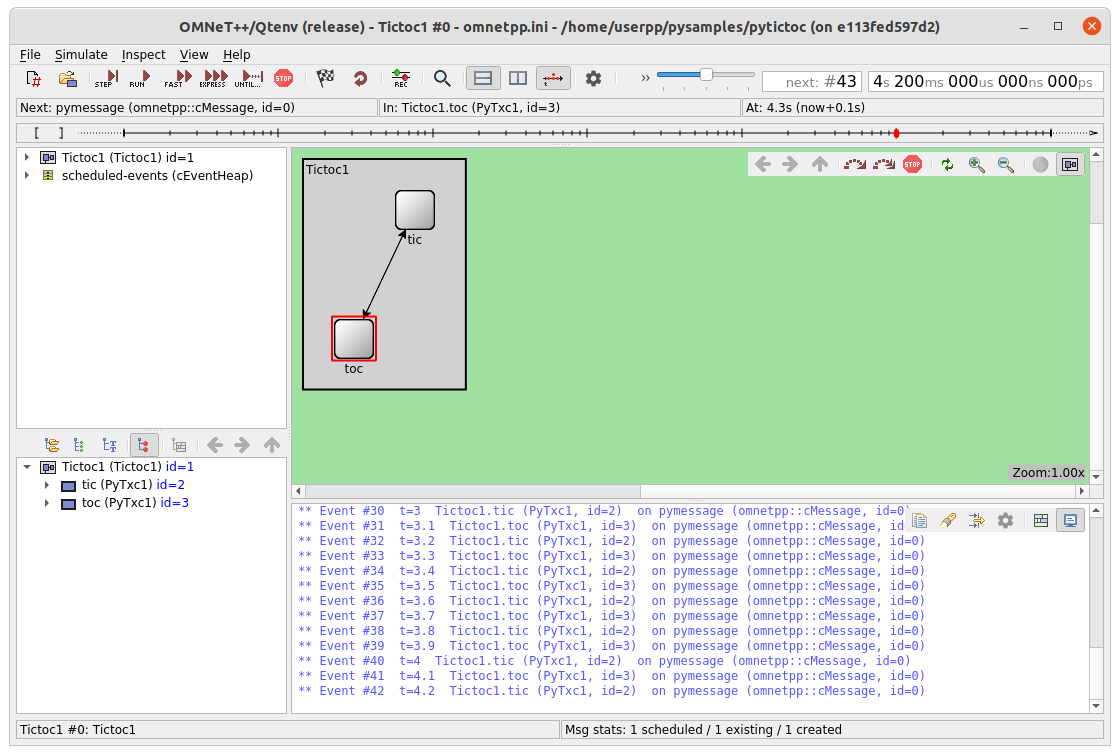
\includegraphics[width=\textwidth]{tictoc}
\end{figure}

Por la sencillez inicial y la complejidad incremental de esta simulación, se
usó como guía de todas las pruebas. Se estableció como primer objetivo poder
escribir los módulos del tutorial tictoc en Python. Esto permitió concentrarse
en las necesidades generales que permitieran la integración funcional de
\omnetpp{} con las clases escritas en Python.

Sólo una vez que se consiguió el objetivo primario, se prosiguió ampliando la
integración para permitir la implementación de módulos de mayor complejidad. En
una segunda etapa, la mayoría de las muestras en el directorio samples fueron
portadas a Python. Asimismo, se implementaron en Python algunos trabajos
prácticos de la cátedra Redes y Sistemas Distribuidos de FaMAF.

\section{Desarrollo}\label{sec:des}
\subsection{Arquitectura de \omnetpp{}}

Tomemos como punto de partida la siguiente definición de módulo simple en C++
(obviando la implementación de los métodos que no son relevantes en este
momento).

\inputminted{c++}{codelistings/txc1.cc}

Luego de compilar de dicho modelo junto al kernel de simulación, el binario
logra crear instancias del módulo \verb!Txc1! (tantas como los archivos NED
indiquen en la descripción de la topología de la red) e invocar a sus métodos.
Nuestro próximo objetivo es entender los mecanismos puestos en juego por
\omnetpp{} para lograr esto. Se exponen a continuación los principales elementos
que contribuyen a entender la solución encontrada.

\subsubsection{El ciclo de vida de una simulación}

Cuando el usuario ejecuta el binario de una simulación el inicio de la
ejecución ocurre en la función main donde únicamente se llama a
\verb!omnetpp::envir::evMain! con los argumentos recibidos del sistema
operativo. En esta última función se llama a \verb!setupUserInterface!,
nuevamente pasando los argumentos de invocación del programa.

Esta función presenta tres etapas claramente señaladas mediante comentarios en
el código:

\begin{enumerate}
    \item SETUP (preparación): procesamiento de la configuración, instanciación
de una interfaz de usuario (gráfica o de consola).

    \item RUN (ejecución): el entorno creado (qtenv, o cmdenv o tkenv) es
efectivamente puesto a correr. Los tres tipos de ambientes comparten mucho
código y terminan llamando a código común en una clase base para correr la
simulación. Aquí se consumen los eventos (mensajes) que los módulos van
generando y enviando. Si se acaban los eventos o se acaba el tiempo designado
para la simulación, esta finaliza.

    \item SHUTDOWN (finalización): limpieza final, antes de devolver el valor
de retorno de la simulación.
\end{enumerate}

Nos interesa particularmente lo que ocurre en las etapas de SETUP y SHUTDOWN,
por lo que podemos obviar los llamados que ocurren en RUN. El siguiente esquema
permite entender mejor lo expuesto y dónde estamos poniendo el foco de
atención.

\subsubsection{Code fragments: ejecución de código genérico}

Existe en \omnetpp{} una clase denominada \verb!CodeFragments!, la cual
analizamos a continuación.

Una instancia de \verb!CodeFragments! se inicializa con dos argumentos:

\begin{enumerate}
    \item un puntero a una función de tipo \verb!void -> void!.
    \item una instancia de un tipo enumerado que representa cuándo debe ser ejecutada tal función:
    \begin{itemize}
        \item \verb!CodeFragments::STARTUP! para designar a las funciones a correr durante la etapa de preparación
        \item \verb!CodeFragments::SHUTDOWN! para designar a las funciones a correr durante la etapa de finalización
    \end{itemize}
\end{enumerate}

A su vez, \verb!CodeFragments! tiene atributos de clase (\verb!head! y
\verb!next!) que sirven para implementar una lista enlazada global. Cada vez
que se inicializa una variable de tipo \verb!CodeFragments! esta se coloca como
cabeza de la lista y almacena un puntero al siguiente elemento (la última de
las instancias que se crearon antes que ella), es decir que se inserta por
delante y hace crecer la lista.  Esta estructura de datos se conoce como
``stack'' o pila.

Existe también la función de clase \verb!CodeFragments::executeAll!, que toma
un tipo (ya sea \verb!CodeFragments::STARTUP! o \verb!CodeFragments::SHUTDOWN!)
y recorre toda la lista, ejecutando las funciones de aquellos
\verb!CodeFragments! que tienen el tipo especificado.

Cerca del inicio de la simulación, durante la estapa de STARTUP se ejecuta

\begin{minted}[linenos=false]{c++}
CodeFragments::executeAll(CodeFragments::STARTUP);
\end{minted}

mientras que cerca del final de la simulación, durante la etapa de SHUTDOWN, se ejecuta:

\begin{minted}[linenos=false]{c++}
CodeFragments::executeAll(CodeFragments::SHUTDOWN);
\end{minted}

Este es un dato muy importante, ya que nos proveerá un mecanismo para manejar el ciclo de vida del intérprete de Python embebido,
lo cual será abordado en la sección~\ref{subsec:interpreterlifecycle}

\subsubsection{El registro global de clases}

A la hora de construir la red para lanzar la simulación, \omnetpp{} va creando
recursivamente los módulos y sus submódulos a partir de su nombre (proveniente
de los archivos NED). Es necesario pasar de un simple string como \verb!"Txc1"!
o \verb!"Tictoc"! a un objeto de la clase apropiada.

Para tal fin, \omnetpp{} cuenta con la clase \verb!cRegistrationList!, la cual
implementa un mapeo de tipo \verb!std::string -> omnetpp::cOwnedObject*!. Para
lograr que tal mapeo sea único y que sea accesible desde cualquier punto del
programa, la clase \verb!cGlobalRegistrationList! implementa una variación del
patrón de diseño conocido como ``singleton''. En efecto, no hay una única
instancia de \verb!cRegistrationList!, si no que hay una especializada para
cada tipo de objeto. En particular, existe una de estas
\verb!cGlobalRegistrationLists! llamada \verb!classes! donde se mapea de
nombres de tipos (por ej, \verb!"Txc1"!, \verb!"Tictoc"!, etc.) a instancias de
\verb!omnetpp::cObjectFactory!.

¿Qué es un \verb!cObjectFactory!? Cada instancia de \verb!cObjectFactory! sabe
cómo crear objetos de un tipo determinado. Almacena una función de creación,
una función de casteo y una descripción en forma de string.

Poniendo todas estas piezas juntas, lo que \omnetpp{} hace para obtener una
instancia de un módulo, en la etapa de construcción de la red (se omite el
manejo de errores):

\begin{itemize}
    \item llama al método de clase \verb!cObjectFactory::createOne(className)!

    \item el método de clase busca en el \verb!cGlobalRegistrationList! llamado
classes a el \verb!cObjectFactory! apropiado para tal nombre de clase

    \item una vez identificado el \verb!cObjectFactory! adecuado, se llama a la
función de creación que este contiene.

\end{itemize}

Todo este andamiaje es transparente para el usuario. Su única responsabilidad
es definir un módulo que herede de \verb!cSimpleModule!, y presentarlo al
sistema mediante \verb!Define_Module!. Todos estos detalles sobre cómo hace
\omnetpp{} para instanciar su clase están ocultos.

Es importante descubrir, entonces, quién provee el \verb!cObjectFactory! que
sabe construir y castear instancias del módulo definido por el usuario, y
además, quién registra ese \verb!cObjectFactory! en la instancia global de
\verb!cGlobalRegistrationList! llamada \verb!classes!.

\subsubsection{El macro \texttt{Define\_Module}}

Luego de la definición de la clase \verb!Txc1!, para su uso en una simulación
es mandatorio escribir \verb!Define_Module(Txc1);!. Sin esta instrucción,
\omnetpp{} simplemente no toma conocimiento del módulo agregado por el usuario.

\verb!Define_Module! parece a simple vista una función, sin embargo es un
macro, cuya definición luce así:

\inputminted{c++}{codelistings/define_module_1.cc}

Esta definición involucra al macro \verb!__REGISTER_CLASS!, que a su vez está
construido sobre otro macro:

\inputminted{c++}{codelistings/define_module_2.cc}

Expandiendo recursivamente todos los macros involucrados (por ejemplo,
utilizando la opción \verb!-E! del compilador) y formateando el espaciado para
mejorar la legibilidad se logra ver que \verb!Define_Module(Txc1);! termina
convirtiéndose en:

\inputminted{c++}{codelistings/define_module_3.cc}

Analicemos un poco el resultado.

\verb!static omnetpp::cObject *__factoryfunc_13()!: define una ``factory
function'', encargada de la creación de nuevas instancias de \verb!Txc1!.

\verb!static void *__castfunc_13(omnetpp::cObject *obj)!: define una función de
casteo, que a partir de un puntero a una instancia de \verb!omnetpp::cObject!
devuelve el resultado de reinterpretar ese puntero como un puntero a instancia
de \verb!Txc1!.

\verb!void __onstartup_func_13()!: define una función que registra ante \omnetpp{}
la existencia de un nuevo tipo de módulo simple llamado \verb!Txc1!, junto con
las funciones de creación y casteo definidas ad hoc.

Se hace notar que los nombres incluyen el número ``13'' porque en el archivo
original, \verb!Define_Module(Txc1)!; estaba escrito en la línea 13. Con esto
se busca diferenciar funciones en el potencial caso de tener diversos usos del
macro \verb!Define_Module! en el mismo archivo. Efectivamente encontramos que,
de ejecutarse la función \verb!__onstartup_func_13!, \omnetpp{} pasaría a tener
conocimiento de un módulo llamado \verb!"Txc1"! y contaría con un mecanismo
para crear instancias del mismo.

Notar que hasta el momento se trata de definiciones de funciones, pero ninguna
de ellas ha sido invocada. Lo que sigue es diferente:

\inputminted{c++}{codelistings/define_module_4.cc}

Esto es una declaración e inicialización de una variable estática de tipo
\verb!omnetpp::CodeFragments! llamada \verb!__onstartup_obj_13! (si bien el
nombre es irrelevante). Al tratarse de una variable estática, su inicialización
ocurre al comenzar la ejecución del programa. Es decir que antes de que la
función \verb!main! sea invocada, esta llamada a constructor ya se ejecutó y
por lo tanto la instancia de \verb!CodeFragments! que se acaba de crear ya se
encuentra formando parte de la lista global de \verb!CodeFragments!. Por lo
tanto, el resultado final de la instanciación de esta variable es la colocación
de \verb!__onstartup_func_13!  de para ser ejecutada durante la etapa de
STARTUP de la función \verb!setupUserInterface!. Más aún, cuando esa función se
ejecute, el resultado es que se registra ante \omnetpp{} un tipo de módulo
simple nuevo (\verb!Txc1!) así como las funciones necesarias para su creación y
casteo. Esto permitirá a \omnetpp{} crear y manipular instancias de \verb!Txc1!
cuando sea necesario (según lo dicten los archivos de descripción de la
topología de la red).

En resumidas palabras, el macro \verb!Define_Module(T)!  (donde \verb!T! es la
clase definida por el usuario) sirve para:

\begin{enumerate}
    \item definir una función (F1) de creación de objetos del tipo \verb!T!

    \item definir una función (F2) de casteo a objetos del tipo \verb!T!

    \item definir una función (F3) que registra ante \omnetpp{} el tipo
\verb!T! junto con las funciones F1 y F2.

    \item definir una variable de tipo \verb!CodeFragments! que al ser estática
se inicializa antes de llamar a la función principal del programa. Esto último
garantiza que F3 se ejecuta durante la etapa de STARTUP de
\verb!setupUserInterface! y, como consecuencia, cuando llega el momento de
instanciar a la clase \verb!Txc1!, \omnetpp{} ya puede hacerlo.

\end{enumerate}

\subsection{Registrando módulos Python}

Luego de conocer el ciclo de vida de la simulación en \omnetpp{}, los mecanismos
que se activan a la hora de declarar un módulo escrito por el usuario (puestos
en juego por el macro \verb!Define_Module!) así como el andamiaje provisto por
\verb!CodeFragments! y las llamadas

\begin{minted}[linenos=false]{c++}
CodeFragments::executeAll(CodeFragments::STARTUP);

CodeFragments::executeAll(CodeFragments::SHUTDOWN);
\end{minted}

\noindent que realiza la función \verb!setupUserInterface!, se empieza a definir una
estrategia para la implementación de módulos directamente en Python.

En una primera etapa, buscamos definir una serie de funciones y definiciones
que hagan en su conjunto lo mismo que el macro anteriormente estudiado.
Convertir todo ese código en un macro lo más sencillo posible sería bueno (para
la comodidad del usuario), pero por el momento se posterga.

Buscamos:

\begin{itemize}
    \item Una función que al ser invocada (sin argumentos) devuelva un puntero
a una instancia de \verb!PySimpleModule! convertido a puntero a instancia de
\verb!cModule!.

    \item Una función de casteo a objetos del tipo \verb!PySimpleModule!.

    \item Una función que sea registrada (como un \verb!CodeFragment!) para ser
ejecutada durante la etapa de SETUP de \verb!setupUserInterface! para registrar
este nuevo tipo ante \omnetpp{}. 

\end{itemize}

A su vez, es necesario inyectar en el ciclo de vida de \omnetpp{} la
inicialización y finalización del intérprete de Python.

Por último, es necesario que el usuario pueda especificar clases en Python
heredando de una clase base que sea la versión Python de \verb!cSimpleModule!,
de forma de poder realizar los casteos a los tipos de C++ que espera \omnetpp{}.

\subsubsection{\texttt{PySimpleModule}: heredando \texttt{cSimpleModule} en Python}

Comenzamos a trabajar en extender el intérprete de Python con las clases de
\omnetpp{}. En una primera etapa se trabajó en exponer sólo aquello que era
estrictamente necesario para lograr la implementación de la primera parte del
tutorial tictoc: las clases \verb!cSimpleModule! con los métodos
\verb!getName! y \verb!send!, y la clase \verb!cMessage!.

También fue en esta etapa en que se trabajó efectivamente con pybind11 por lo
que fue también un momento de exploración de esta herramienta (cuya elección
probó ser acertada).

Se incluye aquí la primera versión exitosa del código que se utilizó para
exponer estas clases, con el objetivo de que el lector tenga noción del tipo de
trabajo que se estaba realizando.

\inputminted{c++}{codelistings/binding.cc}

Luego de la compilación de ese archivo en C++ se obtiene un módulo en Python
que expone las clases \verb!cSimpleModule!, cMessage así como algunos de sus
métodos. Es decir, estamos en condiciones de escribir en Python algo como:

\inputminted{Python}{codelistings/binding_usage.py}

Como puede verse en el siguiente uso interactivo, estas clases no son útiles
fuera del contexto de una simulación:

\begin{minted}[linenos=false]{text}
# python3
>>> from pyopp import cSimpleModule, cMessage
>>> sm = cSimpleModule()
>>> sm.handleMessage(cMessage('hello'))
<!> Error during startup/shutdown: Global simtime_t variable found, with value 0. Global simtime_t variables are forbidden, because scale exponent is not yet known at the time they are initialized. Please use double or const_simtime_t instead. Aborting.
\end{minted}

No obstante, ya contamos con la extensión necesaria para que el código escrito
por el usuario herede en Python de la clase \verb!cSimpleModule! (escrita en
C++). A continuación exploramos cómo integrar estas clases en una simulación.

\subsubsection{Creación de módulos definidos en Python desde C++}

Para lograr que \omnetpp{} sepa cómo instanciar esta clase definida en Python el
paso siguiente fue definir la factory function necesaria. Una primera versión
de la misma luce así:

\inputminted{c++}{codelistings/factory_function.cc}

Esta factory function es esencialmente lo que buscamos, excepto por dos
motivos. El primero de ellos es la conversión intermedia a
\verb!cSimpleModule!, necesaria porque C++ y pybind11 no conocen la relación
entre nuestra clase definida en Python y \verb!cObject!. En una futura versión,
en la que el módulo expuesto a Python incluye toda la jerarquía de clases base
de \verb!cSimpleModule! (la cual tiene a \verb!cObject! en la raíz), este paso
intermedio puede eliminarse.

El segundo motivo, mucho más complejo y difícil de resolver es que al terminar
el scope de la función, el objeto Python que acaba de ser creado es eliminado
de la memoria por el intérprete de Python. Para entender por qué esto es así,
necesitamos hablar de cómo Python maneja la memoria y el ciclo de vida de sus
variables.

Recordemos que en C++, los principales lugares donde las variables pueden
existir son:

\begin{description}
    \item[el stack (manejo automático):] variables declaradas sin manejo
explícito de la memoria y son liberadas tan pronto como salen de scope (el
bloque de código que las contiene). Para alojar una variable en el stack, el
compilador debe conocer su tamaño. Además, el espacio del stack es bastante
limitado.

    \item[el heap (manejo manual):] una fuente mucho mayor de memoria,
administrada por el sistema operativo. Las variables cuya memoria se pide y se
devuelve explícitamente tienen un ciclo de vida independiente del stack y el
compilador no necesita conocer su tamaño.
\end{description}

Naturalmente, Python aloja todos los objetos creados por el usuario en el heap.
A su vez, con el propósito de liberar la memoria de aquellas variables que ya
no se utilizan, cada objeto Python contiene información de cuántas referencias
hay a él en un programa (variables que sirven para alcanzarlo). Digamos que en
el ejemplo:

\begin{minted}[linenos=false]{Python}
a = 'hola'
b = [a]
\end{minted}

El objeto apuntado por la variable a es referenciado en dos lugares (por la
variable \verb!a! y como primer elemento de la lista \verb!b!). Tan pronto como
hacemos:

\begin{minted}[linenos=false]{Python}
b[0] = 'chau'
a = 1
\end{minted}

\noindent el objeto de tipo string \verb!'hola'! que el intérprete de Python
alojó en memoria dinámica ya no es necesario, puesto que no existen referencias
a él. No hay manera de que el programa vuelva a utilizarlo. Es susceptible de
ser eliminado para devolver la memoria al sistema operativo.

El algoritmo que el intérprete utiliza para reconocer este tipo de situaciones
(cuándo es momento de destruir un objeto y devolver su memoria) se conoce como
``reference counting''. Básicamente consiste en incrementar la cuenta cada vez
que se crea una referencia y decrementarla cuando se destruye o sobreescribe
una referencia. Cuando la cuenta se vuelve cero el objeto se puede borrar. No
existen garantías de que el objeto sea borrado inmediatamente, pero el garbage
collector puede hacerlo a partir de ese momento.

Con esta información, no es difícil ver que existe una única referencia al
objeto creado en la línea

\begin{minted}[linenos=false]{c++}
 py::object obj = py_module.attr("PyTxc1")();
\end{minted}

Tan pronto como la variable \verb!obj! (que apunta a un objeto Python en el
heap pero está en el stack) sale de scope y es destruida, el intérprete
reconoce que ya no hay variables apuntando a dicho objeto (desconoce el casteo
a \verb!cSimpleModule*! o \verb!cObject*!) y lo borra (devuelve la memoria al
sistema operativo). Por su lado, el programa \omnetpp{} continúa utilizando la
referencia \verb!ret! que ahora apunta a memoria que es del sistema operativo.
Tan pronto como trate de dereferenciarla, tendremos un \verb!Segmentation Fault!
y el sistema operativo terminará el programa.

La solución implementada fue sencillamente incrementar el contador de
referencias de forma manual antes de que termine la función. 

\begin{minted}[linenos=false]{c++}
    // Instanciamos la clase, obteniendo un py::object
    py::object obj = py_module.attr("PyTxc1")();
    obj.inc_ref();
\end{minted}

Esto evita que el intérprete devuelva la memoria al sistema operativo y permite
que \omnetpp{} utilice la referencia devuelta por la función sin incurrir en un
comportamiento ilegal.

Sin embargo, esto genera un problema simétrico: ahora el objeto Python no será
liberado nunca. Incluso cuando C++ destruya la instancia de cObject que le
devolvimos, el objeto Python seguirá existiendo, ya sin referencias asociadas a
él. Para evitar esto se procedió a decrementar el contador de referencias en el
destructor de la clase base que expusimos a Python:

\begin{minted}[linenos=false]{c++}
~PycSimpleModule() {
    py::object obj = py::cast(this);
    obj.dec_ref();
} 
\end{minted}

Irónicamente, el código del módulo generado por pybind11 se da cuenta de el
objeto C++ que se está borrando es un wrapper a un objeto Python. Al llegar a
cero la cuenta de referencias de dicho objeto, el wrapper debe ser eliminado
también. Este sería el comportamiento correcto si el programa principal fuera
Python y se están invocando librerías escritas en C++. En nuestro caso, es un
``double delete'' o un segundo intento de borrar el objeto.

Borrar un objeto que ya ha sido borrado y cuya memoria ya ha sido devuelta al
sistema operativo es lo mismo que intentar borrar (liberar) una porción de
memoria que ya no nos pertenece. Es otra falta que se penaliza con la
terminación inmediata del programa.

Afortunadamente para nosotros, pybind11 provee un mecanismo para generar código
que no invoca al destructor del objeto C++ una vez que el objeto Python es
liberado.

En resumidas cuentas, el problema se solucionó aplicando las siguientes reglas:

\begin{enumerate}
    \item La cuenta de referencias del objeto Python creado en la factory
function que será llamada por \omnetpp{} debe ser incrementada manualmente,
para evitar que el intérprete decida liberar su memoria tan pronto como la
función retorna.

    \item Cuando \omnetpp{} libera el objeto C++ que en realidad es el wrapper
de un objeto Python, la cuenta de referencias del objeto Python debe ser
decrementada para permitir que su memoria sea liberada.

    \item Pybind11 no debe eliminar el objeto C++ que envuelve al objeto Python
cuando este último sea liberado.
\end{enumerate}

Este problema del ciclo de vida de los objetos volverá a aparecer más adelante
con los mensajes que se crean en un módulo con destino a otro módulo. El
escenario es ligeramente diferente y la solución encontrada, también. Se lo
describe más adelante.

\subsubsection{La función de casteo}

El único uso que se hace de la función de casteo es en el método de
\verb!cObjectFactory!

\begin{minted}[linenos=false]{c++}
/**
* Returns true if the given object can be cast
* (via dynamic_cast) to the class represented by
* this factory object, and false otherwise.
*/
virtual bool isInstance(cObject *obj) const  {
    return castFunc(obj)!=nullptr;
}
\end{minted}

el cual utiliza la posibilidad o imposibilidad de castear el objeto a la clase
declarada como signo de que el objeto en cuestión es o no es instancia de la
misma. Nuestra primera versión de la función de casteo es:

\begin{minted}[linenos=false]{c++}
static void *F2(omnetpp::cObject *obj) {
    return (void*)dynamic_cast<PycSimpleModule*>(obj);
}
\end{minted}

Notar que esta función devolverá \verb!true! para cualquier objeto que haya
sido implementado en Python heredando de \verb!cSimpleModule!. No sirve para
identificar las clases derivadas en Python.

No obstante, no seguimos trabajando en una función de casteo más elaborada por
considerarlo innecesario. Inspeccionando el código de \omnetpp{} se puede
constatar que la función \verb!isInstance! se llama sólamente para validar el
tipo del tercer argumento de la función cComponent::emit. Dicho tercer
argumento es de tipo \verb!cObject*! y tiene como valor por defecto nullptr. No
encontramos ejemplo de su uso en la documentación ni en ninguno de los samples.

\subsubsection{Ciclo de vida del intérprete}\label{subsec:interpreterlifecycle}

Resta proveer un mecanismo que asegure que un intérprete de Python está vivo
durante el tiempo que esto es estrictamente necesario. Es decir, desde antes de
la primera instanciación de nuestros módulos hasta después de la destrucción
del último de ellos.

Se logró instanciando un \verb!pybind11::scoped_interpreter! (sólo uno) que se
mantiene vivo a lo largo de toda la aplicación.

\begin{minted}[linenos=false]{c++}
class InterpreterManager {
  private:
    static void* interpreter;
  public:
    static void ensureInterpreter();
};
\end{minted}

La implementación de \verb!ensureInterpreter! simplemente valida que
\verb!interpreter! sea un puntero nulo (lo cual sirve para identificar la
primera vez que llaman a la función).

Una solución alternativa podría ser agregar la línea

\begin{minted}[linenos=false]{c++}
pybind11::scoped_interpreter guard{};
\end{minted}

\noindent al comienzo de la función \verb!main! de \omnetpp{}.  Esta solución
no nos seduce porque queremos dejar el código original de \omnetpp{} lo más
intacto posible.

\subsubsection{Juntando todas las piezas}

En resumidas cuentas, este es el código que hay que escribir para que \omnetpp{}
levante nuestra implementación del módulo desde un archivo Python:

\inputminted{c++}{codelistings/omnetpy.cc}

\subsubsection{El macro \texttt{Define\_Python\_Module}}

No es difícil ver que el código anterior, necesario para registrar módulos
Python, es esencialmente siempre el mismo, con excepción del nombre del módulo
así como el nombre del archivo donde este vive.

Con el objetivo de facilitar el registro de módulos hechos en Python, en
paralelo al macro \verb!Define_Module!, se creó un macro
\verb!Define_Python_Module!. En esencia, esto es todo el código C++ que un
usuario debe escribir para lograr el mismo resultado que en el ejemplo
anterior:

\inputminted{c++}{codelistings/pytxc.cc}

Donde la clase \verb!PyTxc! está definida en el archivo \verb!txc.py!, y se
asume que el mismo importable (esto es, \verb!import txc! no produce errores).

\subsection{Generalización}

Con el desarrollo presentado hasta aquí en esta sección, queda logrado el
objetivo de hacer que \omnetpp{} instancie clases definidas en Python y las acepte
como implementación de módulos de una simulación. El trabajo hecho para
extender el intérprete (exponer las clases de C++ como módulos Python) incluyó
lo mínimo necesario para poder correr las versiones más simples del tutorial
oficial tictoc. 

A continuación, se prosiguió escribiendo en Python el resto del tutorial
tictoc. Este tutorial tiene unas 17 simulaciones progresivamente más complejas
(aún sobre la idea de dos módulos que se intercambian el mismo mensaje).

En cada iteración se fueron agregando nuevas funcionalidades que debían ser
expuestas a Python (es decir, los bindings debían ser extendidos para incluir
más código de \omnetpp{} y hacerlo accesible desde Python).

Algunas nuevas funcionalidades se resolvieron simplemente agregando una
definición en el módulo de los bindings, otras presentaron desafíos mayores
(borrado de mensajes, logging).

Poco a poco, los principales features de \omnetpp{} fueron soportados en un módulo
Python:

\begin{itemize}
    \item recolección de parámetros desde los archivos de configuración
    \item logging (el macro \verb!EV!)
    \item emisión de señales
    \item manipulación de gráficos en la UI
    \item \verb!WATCH!
\end{itemize}

Luego de concluir las simulaciones propuestas en el tutorial tictoc se comenzó
a implementar en Python las simulaciones provistas en el directorio samples
(contiene diversos ejemplos diseñados para mostrar el potencial de la
herramienta). Esto permitió seguir ampliando la superficie de código expuesta a
Python.

Asimismo, se encontraron algunas limitaciones para las cuales no se encontró
una solución, las cuales se encuentran detalladas en la
sección~\ref{subsec:lim}.

\subsubsection{Mas allá de \texttt{cSimpleModule} y \texttt{cMessage}}

Las clases de \omnetpp{} más elementales para una simulación son las dos
mencionadas en el título. \verb!cSimpleModule! es la clase que el usuario debe
extender para construir sus agentes de simulación, y \verb!cMessage! es la clase
utilizada para producir eventos que empujen el desarrollo de la simulación.
Estas son las únicas clases empleadas en las primeras versiones del tutorial
tictoc y, por lo tanto, fueron las primeras que se expusieron a Python en una
primera etapa exploratoria. Una vez que se vio que el enfoque adoptado fue
exitoso, se procedió a exponer a Python una mayor superficie de la librería de
simulación de \omnetpp{}. Qué exponer y en qué orden fue organizado en torno a
desarrollar en Python los mismos ejemplos que se proveen en el directorio
\verb!samples! del proyecto original. Esto permitió también ir comparando los
resultados de las simulaciones hechas en C++ con las simulaciones hechas en
Python.

Este proceso de migración paulatina de los ejemplos (samples) a Python permitió
enriquecer notablemente el rango de posibilidades de la librería \verb!pyopp!
(el binding expuesto a Python), añadiendo funcionalidad esencial para un
simulador de eventos discretos:

\begin{itemize}
    \item recolección de métricas (clases \verb!cStatistic!, \verb!cStdDev!,
\verb!cAbstractHistogram!, \verb!cHistogram!, \verb!cHistogramStrategy!,
\verb!cOutVector!),

    \item acceso al tiempo de simulación (clase \verb!cSimTime!),

    \item manipulación de la representación gráfica de la simulación (clases
\verb!cCanvas!, \verb!cDisplayString!)

    \item parametrización de experimentos (clase \verb!cPar!)

    \item cambios dinámicos en la organización del modelo (clase
\verb!cTopology!, \verb!cGate!, \verb!cChannel!, \verb!cDataRateChannel!)
\end{itemize}

\subsubsection{El macro \texttt{EV}}\label{subsec:ev}

Existe en \omnetpp{} algo que luce como un objeto (aunque es en realidad un macro)
que sirve para generar mensajes desde el código. Estos mensajes se verán en la
interfaz gráfica de la simulación en un tablero especial destinado a tal fin.

Por ejemplo, el siguiente código (samples/aloha/Host.cc):

\begin{minted}[linenos=false]{c++}
EV << "generating packet " << pkname << endl;
\end{minted}

\noindent produce este efecto en la simulación (ver sección inferior derecha de
la fig.~\ref{fig:aloha_EV}).

\begin{figure}[h]
\caption{Uso de \texttt{EV} en simulación aloha}
\label{fig:aloha_EV}
\centering
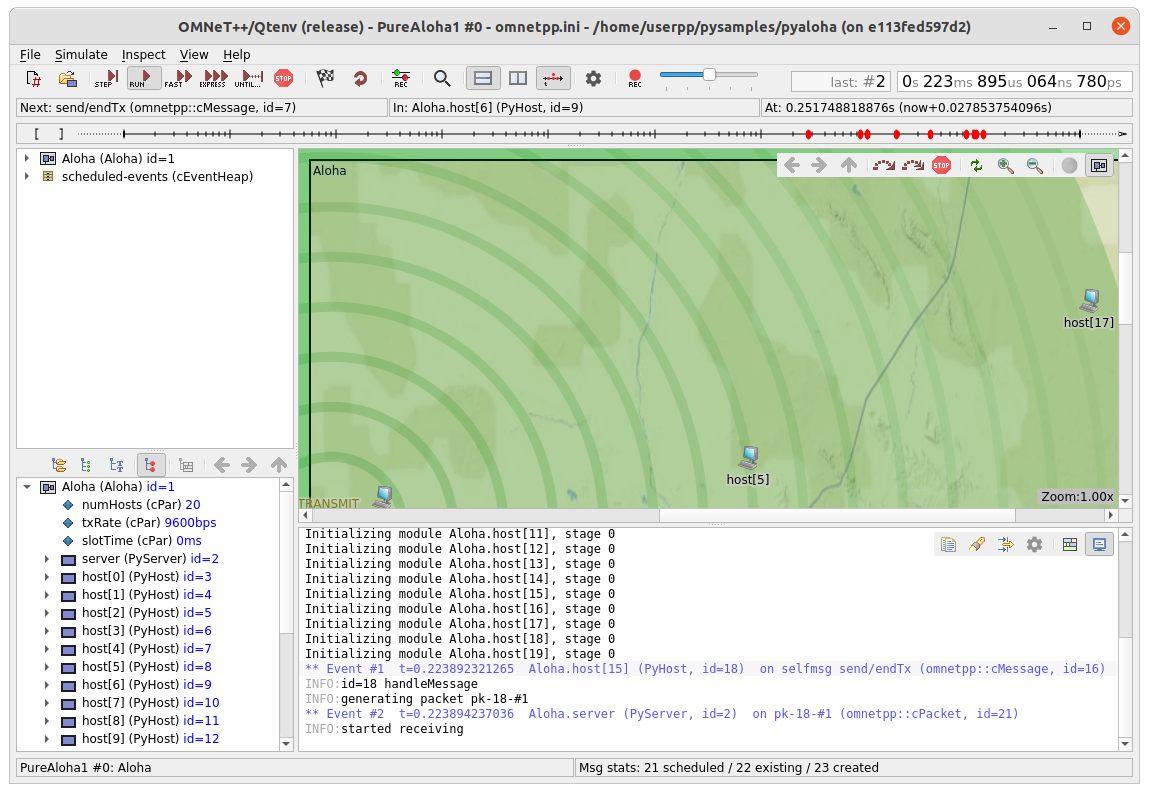
\includegraphics[width=\textwidth]{aloha_EV}
\end{figure}

Este macro hace mucho más que simplemente aceptar una cadena de caracteres:
captura el contexto de quién envía el mensaje, de forma que en la interfaz
gráfica se pueden filtrar mensajes por su origen, como se aprecia en la
figura~\ref{fig:aloha_filter}

\begin{figure}[h]
\caption{Filtrado de mensajes}
\label{fig:aloha_filter}
\centering
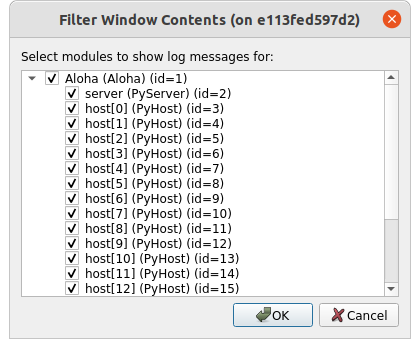
\includegraphics[width=6cm]{aloha_filter}
\end{figure}

% TODO imagen

A su vez, \verb!EV! es un alias de \verb!EV_INFO!, y existen \verb!EV_WARN!,
\verb!EV_DEBUG!, \verb!EV_DETAIL!, etc.

Al portar esta funcionalidad a Python se buscó que la sintaxis fuera lo más
similar posible:

\begin{minted}[linenos=false]{Python}
from pyopp import EV
...
pkname = "pk-%d-#%d" % (self.getId(), self.pkCounter)
EV << "generating packet " << pkname << '\n'
\end{minted}

Este objeto EV se hace cargo de investigar el stack de Python para descubrir
quién emitió el mensaje y crear así un objeto usando la verdadera API de
\omnetpp{} (oculta al usuario de \verb!omnetpy!, para simplificar).

\subsubsection{\texttt{WATCH}: inspección del estado desde la GUI}

\verb!WATCH! es otra herramienta de \omnetpp{} que apunta a facilitar la
trazabilidad de las simulaciones. Se trata de un mecanismo que permite declarar
interés en observar permanentemente el estado de cierta variable o cierto
atributo de un módulo. Suponiendo que existe la variable \verb!counter!, su uso
desde el código sería sencillamente:

\begin{minted}[linenos=false]{c++}
WATCH(counter)
\end{minted}

Para acceder a la información de la variable en tiempo real desde el entorno
gráfico de la simulación, podemos seleccionar \ui{Inspect $\rightarrow$ Find /
Inspect objects}, y utilizar los filtros disponibles hasta dar con lo que nos
interesa, como se muestra en la figura~\ref{fig:tictoc_inspect}.

\begin{figure}[h]
\caption{Inspección de objetos}
\label{fig:tictoc_inspect}
\centering
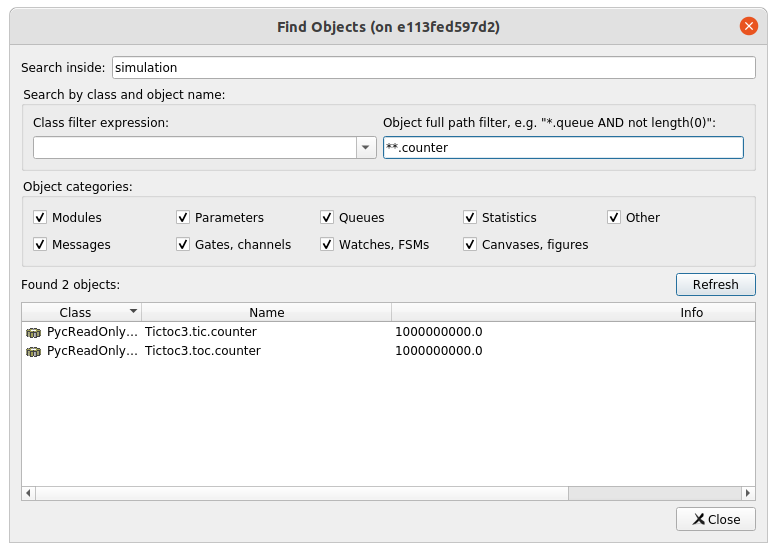
\includegraphics[width=10cm]{tictoc_inspect}
\end{figure}

Esta funcionalidad también se expuso a Python, con la sola diferencia de que
hay que pasar un string con el nombre de la variable que queremos monitorear:

\begin{minted}[linenos=false]{Python}
WATCH('counter')
\end{minted}

\subsubsection{Recolección de estadísticas}

Los datos generados durante una simulación (los sucesivos tiempos de arribo, de
demora, paquetes perdidos, paquetes corruptos, etc.) pueden ser recolectados:

\begin{itemize}
    \item como pares de (tiempo, valor) como una serie temporal
    \item como valores atemporales, utilizados para calcular media, varianza,
etc.
\end{itemize}

Estos datos son recogidos ya sea en cada invocación del método
\verb!handleMessage!, o bien en el método \verb!finish!, el cual se suele
aprovechar para escribir los datos a un archivo en disco.

Los datos generados son escritos en archivos en el subdirectorio results dentro
del directorio de la simulación, y pueden posteriormente ser analizados
utilizando el IDE (entorno de desarrollo integrado).

Las clases necesarias para esta actividad (\verb!cHistogram!,
\verb!cOutVector!) también fueron expuestas a Python.

\subsubsection{El mecanismo de las señales}

\omnetpp{} provee un mecanismo más refinado para la recolección de estadísticas
dentro de una simulación, que permite remover de los módulos el código
específico para registrar los datos en variables o archivos, así como calcular
las diversas medidas de interés antes de finalizar la simulación. Esto brinda
una mayor separación de responsabilidades, y permite que los módulos se
enfoquen en el comportamiento y no en la observación del comportamiento (lo
cual muchas veces cambia según el interés de quien realiza la simulación).

El mecanismo alternativo consiste en señales. Estas tienen un nombre y cada vez
que se emiten, llevan un valor asociado. Quienes estén interesados en observar
el valor de dicha señal se pueden suscribir en los archivos de configuración y
de topología.

Declaración de la emisión de una señal de parte del módulo y de cómo debe ser
escuchada (NED):

\begin{minted}[linenos=false]{text}
simple Txc16
    {
        parameters:
            @signal[arrival](type="long");
            @statistic[hopCount](
                title="hop count";
                source="arrival";
                record=vector,stats;
                interpolationmode=none);
            @display("i=block/routing");
\end{minted}

Declaración de la variable de tipo \verb!simsignal_t! (C++):

\begin{minted}[linenos=false]{c++}
class Txc16 : public cSimpleModule
    {
      private:
        simsignal_t arrivalSignal;
                // ...
\end{minted}

Emisión de un valor para dicha señal (C++):

\begin{minted}[linenos=false]{c++}
void Txc16::handleMessage(cMessage *msg)
    {
        TicTocMsg16 *ttmsg = check_and_cast<TicTocMsg16 *>(msg);
    
        if (ttmsg->getDestination() == getIndex()) {
            // Message arrived
            int hopcount = ttmsg->getHopCount();
            // send a signal
            emit(arrivalSignal, hopcount);
\end{minted}

Sobreescritura de los valores por defecto (qué recolectar y qué ignorar)
(archivo ini):

\begin{minted}[linenos=false]{text}
[Config Tictoc16]
    network = Tictoc16
    **.tic[1].hopCount.result-recording-modes = +histogram
    **.tic[0..2].hopCount.result-recording-modes = -vector
\end{minted}

Esta funcionalidad también se expuso en la librería de Python.

\subsection{Limitaciones y dificultades}\label{subsec:lim}

En esta sección se detallan algunos problemas encontrados durante el desarrollo
del proyecto. Algunos de los mismos no han sido solucionados o su solución
siempre pareció pasajera.

\subsubsection{Ciclo de vida de un mensaje}

Un mensaje dentro de una simulación \omnetpp{} es una instancia de \verb!cMessage!
(u otra clase derivada de \verb!cMessage!, como \verb!cPacket! o cualquier
clase definida por el usuario que tenga a cMessage entre sus clases base).

El mensaje no sólo es importante en tanto y en cuanto permite ``desarrollar la
acción'' dentro de una simulación, sino que también es el combustible que hace
avanzar el código del kernel de \omnetpp{}. En efecto, cuando un módulo ejecuta
su método \verb!send!, el mensaje se encola como un evento a ser procesado por
el kernel de la simulación. Cuando no hay más eventos que procesar, la
simulación termina.

Existe en \omnetpp{} cierto protocolo en relación a quién se hace cargo de
destruir los mensajes (liberar su memoria). En cualquier momento, todo mensaje
tiene un \textit{dueño} (puede ser el módulo que lo está creando, el propio
kernel de la simulación, el módulo que lo recibe). Es el dueño del mensaje el
único habilitado para liberar su memoria.

Cualquier intento de salirse de este protocolo es penado por \omnetpp{}: se paga
con la finalización temprana de una simulación. En el otro extremo, si al
llegar a la finalización de una simulación resulta que hay mensajes que nadie
ha borrado, el sistema emite por pantalla numerosas advertencias de que nadie
se está haciendo cargo de borrar los mensajes que ya no se utilizan:

\begin{minted}[linenos=false]{text}
undisposed object: (omnetpp::cMessage) HypercubeNetwork.node[6].rte.event -- check module destructor
\end{minted}

¿Cómo interactúa este protocolo creación y borrado de mensajes con el manejo
automático de la memoria y el conteo de referencias que hace Python? ¿Cómo
hacemos que nuestros módulos implementados en Python entren a este escenario
sin romper las reglas? ¿Cómo le damos a un módulo implementado en Python la
posibilidad de borrar un mensaje definitivamente? Analicemos lo que sucede en
nuestro ejemplo habitual:

\inputminted{Python}{codelistings/txc1.py}

Es claro que la variable local msg es la única referencia al mensaje creado. Al
finalizar esta función, el algoritmo de conteo de referencias de Python actuará
y se eliminará el objeto. Esto ocasionará el borrado del objeto que existe del
lado de C++. En este momento, \omnetpp{} se quejará de que el mensaje aún no debía
ser borrado, dado que este está en el kernel de la simulación. Fin del
programa.

Para evitar esto, se recurrió a una solución en Python puro. Se hizo un wrapper
de la clase \verb!cMessage! cuyo inicializador guarda una referencia extra al objeto
en un objeto externo denominado \verb!RefStore !(almacén de referencias). De esta
forma, cada vez que se crea un mensaje existen a él dos referencias:

\begin{itemize}
    \item la referencia local (como la variable \verb!msg! en el ejemplo
anterior),

    \item la referencia extra almacenada en \verb!RefStore! por el constructor
de \verb!cMessage!.
\end{itemize}

De este modo, al finalizar la función \verb!initialize! la referencia local se
pierde, pero el mensaje no es eliminado gracias a que aún existe una referencia
(desde el punto de vista de Python). 

Simétricamente, para realizar la tarea de limpieza y liberación definitiva del
mensaje, agregamos a la clase \verb!cSimpleModule! (nuevamente, en Python) la
posibilidad de borrar esta referencia extra mediante el método delete que
acepta un mensaje y trata de quitarlo del \verb!RefStore!, eliminando la última
referencia existente.

Este escenario (Python crea una variable, se la pasa a \omnetpp{}, \omnetpp{}
espera que esa referencia apunte a un objeto durante algún tiempo, Python borra
el objeto apenas termina el bloque de código) se repite en algunos otros
lugares. Allí donde se descubrió que esto sucedía, la solución fue implementar
un wrapper en Python del método original para asegurar la existencia de una
referencia extra al objeto en cuestión. Esta no es la solución ideal, no
obstante, porque a diferencia de lo que ocurre con los mensajes, otro tipo de
objetos no suelen ser explícitamente eliminados en el código Python.

\subsubsection{El método \texttt{deleteModule}}

Existe en \omnetpp{} la posibilidad de que un módulo se declare listo para ser
eliminado de la red: debe ejecutar su método \verb!deleteModule!. Esto permite la
creación de simulaciónes con una topología dinámica. El manejo que hace \omnetpp{}
de esta situación involucra un uso no trivial de excepciones en C++ como forma
de control de flujo. Este método probó ser un verdadero desafío para ser
portado y utilizado desde Python. Finalmente se excluyó de la lista de features
portadas. Esto implica, por ejemplo, que no pudimos implementar el ejemplo
llamado dyna en Python.

\subsubsection{Automatización de la creación de bindings}

El proceso de creación de bindings fue manual. En general, esta actividad se
resistió a una automatización fácil por el hecho de que para cada método de
cada clase expuesta a Python hubo que razonar sobre el uso de los parámetros,
si se usaba paso por referencia o por valor, si Python debía hacerse cargo de
borrar los argumentos o si \omnetpp{} esperaba que estos siguieran vivos luego de
la llamada.

Este proceso en sí es una limitación del proyecto, ya que es propenso a
errores, es lento, y en cada nueva versión de \omnetpp{} habría que hacer una
revisión de todos las clases que se han agregado o que han sufrido alguna
modificación en su interfaz.

Una línea interesante de trabajo futura sería, entonces, el intento de
automatizar la creación de los bindings para Python, complementado con alguna
suite de tests que hicieran uso del módulo Python generado, apuntando a tener
100\% de cubrimiento.

\subsubsection{Mayor cubrimiento de la librería original}

Como se mencionó previamente, se eligió exponer a Python aquello que fue siendo
necesario para migrar las simulaciones de ejemplo del directorio \verb!samples! del
proyecto original. Esto no es el 100\% de la librería de simulación. Notar que
tampoco es deseable exponer cada clase y cada función de \omnetpp{} al mundo de
Python, sino sólo aquellas que un usuario podría llegar a requerir a la hora de
hacer una simulación.

\subsubsection{Depuración}

El IDE de \omnetpp{} habilita la compilación de las simulaciones con símbolos de
debugging (depuración). También permite también el seteo de puntos de debugging
así como entrar a modo debugging si la aplicación termina inesperadamente. Las
funciones de debugging (recorrer código, entrar a funciones, inspeccionar
variables, registros) están perfectamente incorporados a la interfaz gráfica
del IDE (que como ya se ha dicho, está construido encima de Eclipse).

Al implementar módulos en Python, muchas de estas funcionalidades quedan
obsoletas, o se están perdiendo definitivamente. Si la simulación que se está
debuggeando tiene módulos implementados en Python, al llegar el momento de
llamar a una función implementada en Python, el debugger de C++ no ve un cambio
de lenguaje, simplemente nos ofrece entrar al código del intérprete de Python
(hecho en C). Esto, asumiendo que la versión de Python con símbolos de
debugging está disponible en el sistema y ha sido apropiadamente enlazada a la
simulación (durante la compilación).

Nuestro proyecto no se provee compilación con símbolos de debugging de nuestro
código ni una versión de las librerías de Python con símbolos de debugging. Aún
si estos estuvieran disponibles, sería interesante que la ejecución del
debugger permitiera entrar al código Python utilizando pdb (y no gdb).

\subsubsection{La función de casteo}

Dentro del macro \verb!Define_Python_Module! se provee una función de casteo.
Analizando el código de \omnetpp{} se puede apreciar que esta se usa en última
instancia para poder distinguir si un módulo es una instancia de nuestra clase
o no. En el caso de los módulos definidos en Python, la función de casteo está
devolviendo \verb!true! para todos. Si bien esto no nos trajo dificultades en la
implementación y ejecución de ninguna simulación, sería interesante desarrollar
una mejor función de casteo que permitiera reconocer diversas subclases de
\verb!PycSimpleModule! implementadas en Python.

\section{Omnetpy}\label{sec:omnetpy}

\subsection{Arquitectura del proyecto}

En una primera etapa de trabajo (particularmente durante de investigación de la
arquitectura de software y la ejecución de una simulación) se re realizó
bastante intervención sobre el código propio de \omnetpp{} (con la finalidad de
trazar llamadas, imprimir argumentos, etc). Naturalmente, el código propio de
nuestro trabajo (nuevas definiciones, bindings) fue siendo añadido a la
estructura de directorios propuesta por \omnetpp{} (nuevos encabezados en el
directorio \verb!include!, nuevas fuentes en el directorio \verb!src!, etc).
Con el objetivo de compilar \omnetpp{} así como los Python bindings en el mismo
proceso, también se realizaron modificaciones sobre el \verb!Makefile! de
primer nivel.

Con el tiempo, este enfoque fue dejando ver algunas limitaciones ya que las
modificaciones que fueron hechas para \omnetpp{} 5.5.1 no necesariamente se
dejaban aplicar de forma directa sobre otras versiones. En particular, nos
interesó probar nuestros cambios sobre \omnetpp{} 6, que incluye soporte para
editar archivos Python directamente en el IDE (resaltado de sintaxis,
autocompletado, etc.). Si bien no es imposible aplicar los cambios sobre otras
versiones de \omnetpp{}, requiere supervisión manual. En particular, la edición
del \verb!Makefile! (para forzar el compilado de nuestro código junto con el
resto del proyecto) probó ser un mecanismo difícil de automatizar.

Prácticamente estábamos obligados a seguir utilizando los Python bindings con
la versión de \omnetpp{} inicialmente elegida (5.5.1) o elegir para nuestro
proyecto una estructura de versiones que fuera espejo de las de \omnetpp{}, y
realizar adaptaciones particulares para cada una.

Con el fin de simplificar el proceso de integración se comenzó a separar
nuestro trabajo en un proyecto independiente que pudiera ser aplicado
prácticamente sin cambios a distintas versiones de \omnetpp{}. Comenzamos a
utilizar el término ``omnetpy'' para referirnos al conjunto de los archivos
agregados por nosotros.

\subsection{Separando omnetpy de \omnetpp{}}

Dado que nosotros controlamos el ambiente de trabajo de forma prácticamente
total (mediante el uso de imágenes docker), aislar nuestros cambios y
compilarlos de forma independiente en un proceso automático probó ser una tarea
bastante sencilla y con beneficios inmediatos.

En una primera etapa se compila el proyecto \omnetpp{} (la versión elegida, no
importa cuál sea) y luego se compila omnetpy.

Esta es la estructura de directorios de nuestro proyecto:

\begin{itemize}
    \item bindings: código para la generación de la librería Python pyopp

    \item bindings/pyopp: definición Python pura del módulo pyopp

    \item include: encabezados C++ (\verb!Define_Python_Module!, definición de
\verb!PycSimpleModule!, definición de \verb!InterpreterManager!)

    \item lib: tras el proceso de compilación, aquí se deja la librería C++
\verb!libomnetpy.so!. Esta debe enlazarse a cualquier binario que desee
    \item utilizar el macro \verb!Define_Python_Module!.

    \item src: código C++ (implementación de \verb!InterpreterManager!)
\end{itemize}

Luego de esta separación, se probó con éxito la integración de nuestro código
sobre diversas versiones de \omnetpp{} (5.6.1, 6.0.pre6).

Por supuesto, si una versión de \omnetpp{} cambia la API de las clases que
nosotros deseamos exponer a Python, nuestro código debe también ser diferente.
No estamos tomando esas pequeñas diferencias en cuenta. Esto sí obligaría a
generar Python bindings ajustados a cada versión de \omnetpp{} (ya sea de forma
manual o automática).

\subsection{El módulo \texttt{pyopp}}

La compilación de los archivos \verb!bind_<clase de OMNeT++>.cc! y su posterior
enlazamiento produce un módulo Python cuyo nombre completo es (dependiendo de
la versión de Python) \verb!_pybind.cPython-37m-x86_64-linux-gnu.so!. Si bien
este módulo se puede importar desde Python, preferimos agregar una capa hecha
completamente en Python que realiza algunas adaptaciones. Así, el módulo que
importa el usuario (\verb!pyopp!) es un wrapper que elige qué y cómo exponer
del módulo hecho en C++.

\subsection{Compilación del proyecto}

El proyecto cuenta con algunos archivos escritos en C++ que necesitan ser
compilados

\begin{description}
    \item[para la extensión del intérprete:] estos archivos son compilados y
enlazados con las librerías de desarrollo de Python, produciendo un módulo que
se puede importar desde Python.

    \item[para embeber el intérprete:] estos archivos no son parte del módulo
de extensión, si no que se encargan de que \omnetpp{} inicialice un intérprete
de Python antes de instanciar la primera clase definida en Python.
\end{description}

Estos archivos son compilados utilizando un \verb!Makefile! que resuelve todos
los detalles de enlace, encabezados, flags necesarios, etc. Este paso, además,
es realizado como parte de la generación de la imagen Docker que se usó para
desarrollar el trabajo.

\subsection{Manual de usuario}

El uso de \omnetpp{} con omnetpy es muy similar a su uso sin omnetpy. Sólo hay que
realizar algunos pasos extra, como por ejemplo:

\begin{itemize}
    \item Escribir las clases derivadas de \verb!cSimpleModule! en Python

    \item Escribir un archivo C++ utilizando el macro
\verb!Define_Python_Module!

    \item Asegurarse que al compilar el proyecto sean incluidos los encabezados
de omnetpy (por ej, donde se define el macro mencionado).
\end{itemize}

Se incluye a continuación una guía paso a paso que muestra al usuario cómo
realizar una simulación usando \omnetpp{} con omnetpy, desde el IDE.

\subsubsection{Prerrequisitos}

Se asume la disponibilidad de:

\verb!git! (para clonar el proyecto)

\verb!make! (para evitar el tipeo de comandos muy largos)

\verb!docker! (para construir imágenes y lanzar contenedores)

X11 socket (para lanzar aplicaciones con entorno gráfico desde docker)

\subsubsection{Opción 1: generar imagen docker}

Clonar el repositorio del proyecto:

\begin{minted}[linenos=false]{text}
git clone https://github.com/mmodenesi/omnetpy.git
\end{minted}

Generar una imagen docker:

\begin{minted}[linenos=false]{text}
make build
\end{minted}

En este punto se puede especificar la versión de \omnetpp{} que se desea utilizar, por ejemplo:

\begin{minted}[linenos=false]{text}
OMNETPP_VERSION=5.6 make build
\end{minted}

Se espera que la versión sea descargable desde la página de releases de
\omnetpp{}, de lo contrario, la creación de la imagen fallará. Consultar la lista
de versiones disponibles en https://github.com/omnetpp/omnetpp/releases

Lanzar un contenedor:

\begin{minted}[linenos=false]{text}
make run
\end{minted}

Notar que el comando que se ejecuta en este target de \verb!make! lanza un
contenedor efímero en el cual se monta el directorio actual del host en
/home/userpp/workspace. Esto quiere decir que al salir del contenedor este será
eliminado, pero los archivos creados en el directorio /home/userpp/worspace
serán visibles en el host. Alternativamente, si el usuario desea montar otro
directorio, o desea que el contenedor no sea efímero, se sugiere ejecutar
\verb!make run -n! para ver el comando y ejecutar una versión modificada
apropiadamente.

\subsubsection{Opción 2: utilizar una imagen pregenerada}

Alternativamente, es posible utilizar una de las imágenes de docker
pregeneradas y listadas en https://hub.docker.com/r/mmodenesi/omnetpy

Por ejemplo:

\begin{minted}[linenos=false]{text}
docker run \
    --rm -ti \
    -e DISPLAY=$DISPLAY -v /tmp/.X11-unix:/tmp/.X11-unix \    
    mmodenesi/omnetpy:ub18.04_opp5.6.2 bash
\end{minted}

El nombre de la imagen anuncia qué versión de ubuntu y qué versión de \omnetpp{}
se utiliza. El ejemplo anterior está utilizando una imagen construida a partir
de ubuntu:18.04 y con \omnetpp{} 5.6.2.

\subsubsection{Escribiendo una simulación con omnetpy}

Dentro del contenedor, lanzar el IDE

\begin{minted}[linenos=false]{text}
omnetpp
\end{minted}

Cuando levantamos el IDE por primera vez nos pregunta qué directorio
utilizar como ``workspace'' por defecto, como se puede observar en la
figura~\ref{fig:workspace}.

\begin{figure}[h]
\caption{Selección de directorio de trabajo}
\label{fig:workspace}
\centering
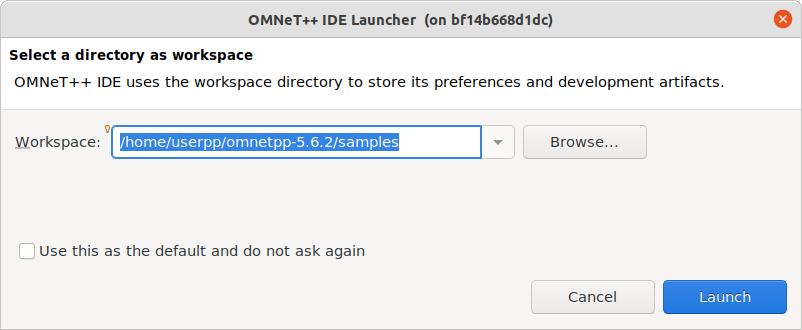
\includegraphics[width=10cm]{workspace}
\end{figure}

Se recomienda usar la ruta /home/userpp/workspace, ya que en general lanzamos
contenedores docker donde esa ruta es un volumen (lo que hacemos desde el
contenedor dentro de ese directorio, se persiste en el host, más allá de la
vida útil del contenedor).

\subsubsection{Preparando un nuevo proyecto}

Desde el IDE, seleccionar \ui{File $\rightarrow$ New $\rightarrow$ OMNeT++
Project} (fig.~\ref{fig:new_project}). Al aparecer el diálogo Wizard, ingresar
\verb!pytictoc! como nombre del proyecto, seleccionar \ui{Empty project} y
luego \ui{Finish}. Un nuevo proyecto aparecerá en el área de proyectos del IDE.

\begin{figure}[h]
\caption{Creación de un nuevo proyecto}
\label{fig:new_project}
\centering
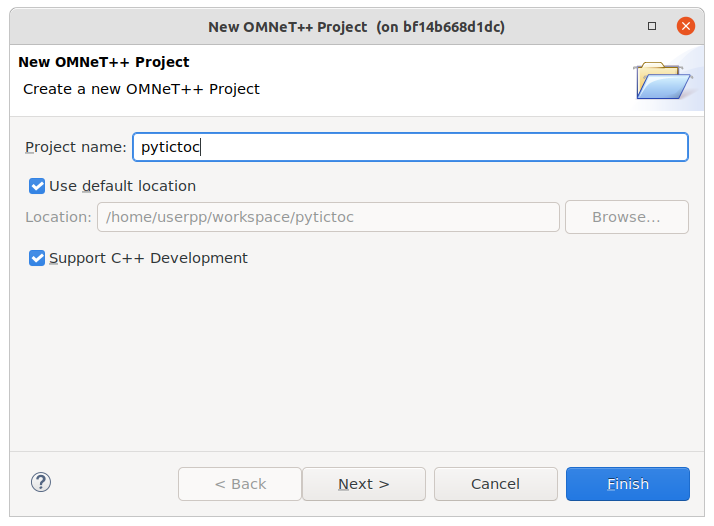
\includegraphics[width=10cm]{new_project}
\end{figure}

\subsubsection{Agregando un archivo NED}

Hacer click derecho en el proyecto y seleccionar \ui{New $\rightarrow$ Network
Description File (NED)}.

% TODO imagen

Guardarlo como \verb!pytictoc.ned! con el siguiente contenido:

\inputminted{text}{codelistings/tictoc.ned}

\subsubsection{Agregando un archivo C++}

Hacer click derecho en el proyecto y seleccionar \ui{New $\rightarrow$ File} y
guardarlo como \verb!txc.cc! con el siguiente contenido:

\inputminted{c++}{codelistings/tictoc.cc}

Dado que el archivo \verb!omnetpy.h! no se encuentra en un directorio conocido
por el IDE, es esperable que se señalen errores en relación a su inclusión o a
\verb!Define_Python_Module!. Para cambiar esto se debe agregar el directorio
\verb!/home/userpp/omnetpy/include! a la lista de directorios escaneados en
busca de archivos de encabezado. En la versión actual del IDE esto se logra en
\ui{Project $\rightarrow$ Properties $\rightarrow$ C/C++ General $\rightarrow$
Path and Symbols} y clickeando el botón \ui{Add}.

\subsubsection{Agregando un archivo \texttt{makefrag}}

Hacer click derecho en el proyecto, seleccionar \ui{New $\rightarrow$ File} y
guardarlo como \verb!makefrag! con el siguiente contenido:

\begin{minted}[linenos=false]{text}
INCLUDE_PATH += $(shell python3 -m pybind11 --include) -I$(OMNETPY_ROOT)/include
LIBS = -lomnetpy $(shell python3-config --libs | cut -d" " -f1)
LDFLAGS += -L$(OMNETPY_ROOT)/lib
\end{minted}

Estas líneas van a ser incluidas en el archivo \verb!Makefile! autogenerado por
\omnetpp{} para compilar la simulación. Es esencial que se llame
\verb!makefrag!.

\begin{quotation}
\noindent\textbf{Nota importante}: si la versión de Python es 3.8 o mayor,\\
\verb!python3-config --libs!\\
debe reemplazarse por\\
\verb!python3-config --libs --embed!.
\end{quotation}

\subsubsection{Agregando un archivo Python}

Hacer click derecho en el proyecto, seleccionar \ui{New $\rightarrow$ File} y
guardarlo como \verb!txc.py! con el siguiente contenido:

\inputminted{Python}{codelistings/tictoc.py}

\subsubsection{Correr la simulación}

En el panel del editor seleccionar el archivo \verb!txc.cc! (la fuente en C++).
Esto es importante para forzar al IDE a ofrecernos la compilación de una
simulación C++ en el siguiente paso.

Seleccionar \ui{Run $\rightarrow$ Run} y elegir \ui{OMNeT++ Simulation}

% TODO imagen

Luego de la compilación, se lanza automáticamente la ejecución de la
simulación:

% TODO imagen

\section{Evaluación}\label{sec:ev}

Se procedió a verificar el funcionamiento de un modelo de \omnetpp{} hecho en
Python. Para realizar esta tarea se implementó la simulación de ejemplo aloha
(parte de la distribución oficial de \omnetpp{}) en Python (la llamaremos
pyaloha).

Se puede mostrar teóricamente que para el protocolo de transmisión aloha el uso óptimo del
canal ($\frac{1}{e}$, aproximadamente $18.4\%$) ocurre cuando se emite un paquete cada dos
unidades de tiempo, mientras que para el protocolo aloha ranurado, el uso
óptimo ($\frac{1}{2e}$, aproximadamente $36,8\%$) ocurre cuando se emite un paquete por
unidad de tiempo [42].

\subsection{Verificación}

Para la implementación de pyaloha se siguió un patrón de traducción casi línea
por línea del código original en C++, para evitar introducir cambios
inadvertidos en el modelo.

Se ejecutó la simulación con los siguientes parámetros:

\begin{itemize}
    \item número de hosts: 15

    \item tasa de transmisión: 9600kbps

    \item tamaño de paquete: 952b

    \item tiempo total de simulación: 60min

    \item tiempo entre paquetes: variable exponencial con media $\lambda$,
donde $\lambda$ se hizo variar entre 0 y 15 (segundos)
\end{itemize}

Para el modelo original implementado en C++, se obtuvieron los siguientes
resultados:

% TODO imagen

Para el modelo pyaloha se obtuvieron los mismos resultados. No es que se
obtuvieron resultados similares: se obtuvieron exactamente los mismos
resultados. Recordar que la inicialización del generador de números aleatorios
utiliza la misma semilla, por lo que los eventos han sido generados en tiempos
exactamente iguales, en ambos modelos.

Esto deja claro que la implementación del modelo en Python es tan funcional
como la implementación del modelo en C++.

\subsection{Rendimiento}

A continuación se presenta una comparación entre los modelos realizados con
\omnetpp{} (código en C++) y los mismos modelos escritos en Python, en términos de
velocidad de procesamiento. Las simulaciones se realizaron en una notebook con
procesador Intel i7-1065G7 CPU @ 1.30GHz, con 8GB de memoria RAM. Sin embargo,
los resultados se presentan en términos de eventos por segundo (una métrica que
\omnetpp{} escribe por salida estándar).

\subsubsection{Aloha}

Mientras menor es el tiempo medio entre paquetes, las simulaciones necesitan
más tiempo para finalizar. Esto es debido a que se generan más mensajes
(eventos) que deben ser procesados por el kernel de simulación hasta alcanzar
el tiempo límite de 60 minutos (simulados).

Observamos que la ejecución más lenta del modelo hecho en C++ corre en menos de
un segundo:

% todo imagen

En tanto que para pyaloha, el tiempo alcanzado supera los 3 minutos:

% todo imagen

Independientemente del tiempo medio entre mensajes, del tiempo total de la
simulación o de si el protocolo es ranurado o no, se puede observar que el
modelo implementado directamente en C++ procesa unos $1200000$ eventos por
segundo, mientras que el modelo implementado con Python es unas $200$ veces más
lento, procesando sólo $6000$ eventos por segundo.

\subsubsection{Tictoc}

Para Tictoc1, que consiste en un simple pasaje de mensajes entre dos instancias
de \verb!Txc!, encontramos que el modelo implementado en C++ procesa unos 5
millones de eventos por segundo, mientras que el que utiliza Python sólo
alcanza el medio millón, es decir, es unas 10 veces más lento.

Tictoc2 presenta herramientas para loggear información durante una simulación.
En particular, se introduce el constructo \verb!EV!, que en C++ está
implementado como un macro. En este caso, la performance de C++ no se ve
afectada, alcanzando también unos 5 millones de eventos por segundo. En cambio,
el modelo que utiliza Python sólo alcanza unos 17.000 mensajes por segundos
(unas 300 veces más lento). Esto se debe a que en Python, \verb!EV! no está
llamando directamente a código C++ de \omnetpp{} (que, como se dijo en la
sección~\ref{subsec:ev}, es un macro y por lo tanto es expandido en tiempo de
compilación) si no que es un objeto que inspecciona el stack para conocer el
contexto.

En efecto, si el modelo en C++ dice:

\begin{minted}[linenos=false]{c++}
EV << getName() << "'s counter is " << counter << "\n";
\end{minted}

\noindent su traducción directa a Python resulta aproximadamente 1000 veces más
lenta

\begin{minted}[linenos=false]{Python}
EV << self.getName() << "'s counter is " << self.counter << '\n'
\end{minted}

\noindent mientras que la siguiente variante, aparentemente igual, es sólo 300
veces más lenta

\begin{minted}[linenos=false]{Python}
EV << f"{self.getName()}'s counter is {self.counter}\n"
\end{minted}

La diferencia viene dada por el hecho de que la primera variante (la que es más
lenta) consiste en 4 usos del operador \verb!<<! (left shift) sobre el objeto
\verb!EV!, cada uno de los cuales se traduce en una inspección del stack trace
para evaluar el contexto de ejecución, mientras que en la segunda variante se
utiliza \verb!<<! una única vez.

\subsubsection{Conclusión}

Como era de esperar, se encontró que los modelos implementados directamente en
C++ se terminan de simular más rápidamente. No obstante, qué tanto más rápido
no es un valor constante: la complejidad del método \verb!handleMessage! dicta
la magnitud de la penalidad en la performance. Esto es consistente con el hecho
de que mientras más tiempo pase la simulación ejecutando instrucciones Python
dentro del intérprete, más se aleja de la performance ideal alcanzada por un
modelo que utilice sólo C++ la totalidad del tiempo.

\subsection{Complejidad de código}

La siguiente comparación entre modelos de \omnetpp{} puro (C++) y \omnetpp{}
implementando modelos en Python se basa en la reimplementación de los
siguientes ejemplos de muestra incluidos en el código fuente de \omnetpp{}: aloha,
canvas, cqn, dyna, fifo, histograms, hypercube, routing, tictoc.

En ciertos fragmentos de código donde predomina la llamada a métodos y
funciones de \omnetpp{}, los modelos en C++ y los modelos en Python son
necesariamente casi idénticos, como se observa en el siguiente ejemplo:

routing/builder/netbuilder.cc

\begin{minted}[linenos=false]{c++}
void NetBuilder::initialize()
{
    scheduleAt(0, new cMessage());
}
\end{minted}

pyrouting/pymodules/netbuilder.py:

\begin{minted}[linenos=false]{Python}
    def initialize(self):
        self.scheduleAt(0, cMessage())
\end{minted}

No obstante, notamos algunos factores que contribuyen a una mejora en la
complejidad de código: ausencia de caracteres como corchetes y punto y coma
para estructurar el código, ausencia de calificación del nombre de espacios
(\verb!Netbuilder::!).

En líneas generales, los modelos de ejemplo que incluye \omnetpp{} están diseñados
para mostrar cómo trabajar con \omnetpp{}, lo cual hace que el código consista
principalmente en llamadas a las APIs y, por lo tanto, su implementación usando
Python sea prácticamente igual en términos de cantidad de líneas.

Donde realmente vemos la diferencia es, por ejemplo:

routing/builder/netbuilder.cc

\begin{minted}[linenos=false]{c++}

    std::map<long, cModule *> nodeid2mod;
    std::string line;

    std::fstream nodesFile(par("nodesFile").stringValue(), std::ios::in);
    while (getline(nodesFile, line, '\n')) {
        if (line.empty() || line[0] == '#')
            continue;

        std::vector<std::string> tokens = cStringTokenizer(line.c_str()).asVector();
        if (tokens.size() != 3)
            throw cRuntimeError("wrong line in module file: 3 items required, line: \"%s\"", line.c_str());

        // get fields from tokens
        long nodeid = atol(tokens[0].c_str());
        const char *name = tokens[1].c_str();
        const char *modtypename = tokens[2].c_str();
        EV << "NODE id=" << nodeid << " name=" << name << " type=" << modtypename << "\n";

        // create module
        cModuleType *modtype = cModuleType::find(modtypename);
        if (!modtype)
            throw cRuntimeError("module type '%s' for node '%s' not found", modtypename, name);
        cModule *mod = modtype->create(name, parent);
        nodeid2mod[nodeid] = mod;

        // read params from the ini file, etc
        mod->finalizeParameters();
    }
\end{minted}

Python:

\begin{minted}[linenos=false]{Python}

    nodeid2mod = {}

    with open(self.par('nodesFile').stringValue(), 'r') as fh:
        for line in fh.readlines():
            line = line.strip()
            if not line or line.startswith('#'):
                continue

            nodeid, name, modtypename = line.split()
            nodeid = int(nodeid)

            EV << 'NODE id=' << nodeid << ' name=' << name << ' type=' << modtypename << '\n'

            # create module
            modtype = cModuleType.find(modtypename)
            if modtype is None:
                raise RuntimeError(f'module type '{modtypename}' for node '{name}' not found')

            mod = modtype.create(name, parent)
            nodeid2mod[nodeid] = mod

            # read params from the ini file, etc
            mod.finalizeParameters()

\end{minted}

donde Python es más simple por no declaración de variables, la facilidad de
lectura de archivos, la facilidad para manipulación de strings o, como vemos en
el siguiente ejemplo, por la facilidad para trabajar con diccionarios:

C++:

\begin{minted}[linenos=false]{c++}
    std::map<long, cModule *>::iterator it;

    for (it = nodeid2mod.begin(); it != nodeid2mod.end(); ++it) {
            cModule *mod = it->second;
            mod->buildInside();
    }
\end{minted}

Python:

\begin{minted}[linenos=false]{Python}
        for mod in nodeid2mod.values():
            mod.buildInside()
\end{minted}

Como puede apreciarse en la tabla~\ref{table:loc}, la cantidad de líneas
necesaria para implementar un modelo en Python siempre fue menor que para el
modelo original en C++.  En el análisis se tienen en cuenta únicamente archivos
\verb!.h!, \verb!.cc!, \verb!.msg! y \verb!.py!.

\begin{table}[h!]
\centering
\begin{tabular}{l|rrr}
Modelo & C++ & Python & Proporción\\
\hline

aloha     & 511  & 352  & 68,88\% \\
canvas    & 145  & 114  & 78,62\% \\
cqn       & 185  & 100  & 54,05\% \\
dyna      & 401  & 291  & 72,57\% \\
fifo      & 285  & 122  & 42,81\% \\
histogram & 158  & 139  & 87,97\% \\
hypercube & 368  & 263  & 71,47\% \\
routing   & 551  & 370  & 67,15\% \\
tictoc    & 1755 & 705  & 40,17\% \\
\end{tabular}
\caption{Cantidad de líneas de código en modelos reimplementados en Python}
\label{table:loc}
\end{table}

Además de las características ya mencionadas que hacen de Python un lenguaje
más simple de manejar, los modelos implementados en Python tienen menos
archivos y menos líneas.

\section{Conclusiones}\label{sec:conc}
Se presenta una extensión del simulador de eventos discreto \omnetpp{} que permite
escribir módulos simples en el lenguaje de programación Python. Esto habilita a
la escritura de modelos de simulación sin necesidad de saber programar en el
lenguaje oficial de \omnetpp{}, es decir, C++.

C++ es un lenguaje de programación que provee pocas abstracciones sobre el
hardware subyacente y que se compila para obtener un binario ejecutable
convierten en herramienta muy poderosa para escribir código de alta performance
(administración manual de la memoria, complejo sistema de tipos, posibilidad de
incluir código assembly), hacen de este un lenguaje de difícil dominio y con
tiempos de desarrollo relativamente largos, si los comparamos con otros
lenguajes como Python.

Python es un lenguaje de programación de mucho más alto nivel, donde los
detalles del hardware son alejados del usuario final. Un sistema de tipos más
flexible que requiere menos especificidad por parte del usuario, manejo
automático de la memoria, una sintaxis más cercana al lenguaje natural, hacen
de este un lenguaje muy idóneo para principiantes o para enseñanza en carreras
relacionadas a la computación. Los programas en Python no se compilan, sino que
son consumidos por otro programa (el intérprete de Python) para llevarlos a
instrucciones de la máquina virtual de Python y finalmente ejecutar tales
instrucciones una a una en el CPU. La implementación más popular de intérprete
está hecha en C y se conoce como cPython.

En general, los programas escritos en C++ son varias veces más rápidos que
programas con la misma funcionalidad escritos en Python, y los programas
escritos en Python son más fáciles de entender, modificar, extender. Es decir
que al movernos de C++ a Python, lo que se gana es mayor claridad en el código
y tiempos de desarrollo más cortos, mientras que si nos movemos en la otra
dirección, lo que se gana es mayor performance computacional.

La posibilidad de escribir simulaciones de \omnetpp{} usando Python en lugar de
C++ tiene varias ventajas asociadas:

\begin{itemize}
    \item menor barrera de entrada para usuarios nuevos

    \item mayor facilidad para incorporar \omnetpp{} en cursos de computación

    \item menor tiempo de prototipado de nuevos modelos

    \item inmediata disponibilidad de todos los recursos del ecosistema Python

    \item posibilidad de introducir cambios en el modelo sin pasos extra de
compilación
\end{itemize}

La extensión de la herramienta \omnetpp{} fue realizada sin necesidad de modificar el código fuente original, lo cual facilita su aplicación en distintas versiones de \omnetpp{}.

Las simulaciones ejecutadas con modelos hechos en Python arrojaron idénticos
resultados que las versiones originales en C++, aunque con penalidades de
performance variable (dependiendo de la complejidad del método \verb!handleMessage!).

\subsection{Desafíos abiertos}

Como se menciona en la sección~\ref{subsec:lim} del capítulo destinado a hablar
del desarrollo del trabajo, quedan algunos desafíos abiertos para continuar con
la tarea iniciada en este trabajo, los cuales se detallan a continuación.

\subsubsection{Generación automática de librerías de extensión}

La extensión del intérprete con las librerías de \omnetpp{} se realizó
manualmente y exponiendo sólo aquellas partes que eran necesarias para portar
las simulaciones de ejemplo del proyecto original.

Sería interesante que este proceso fuera automatizado de forma que dada una
versión de \omnetpp{} se generaran los Python bindings de la totalidad de la
librería.

Las ventajas de esto serían:

\begin{enumerate}
    \item Que cualquier función, clase, método, macro, tipo definido en
    \omnetpp{} (en C++) fuera accesible y extensible desde Python

    \item Se podría contar fácilmente con versiones de omnetpy para cualquier
    versión de \omnetpp{} (recordar que el trabajo se basa en la versión 5.6.2 y se
    probó ligeramente sobre las versiones de perview de \omnetpp{} 6).

    \item En caso de emprender este esfuerzo, sería interesante dedicar algún
    tiempo a diseñar una infraestructura de testing. Por ej, realizar simulaciones
    en C++ y en Python y comparar que las salidas de sus ejecuciones sean
    idénticas, apuntando a que estas simulaciones utilicen el mayor porcentaje
    posible de las librerías.
\end{enumerate}

\subsubsection{Depurador interactivo en Python}

Actualmente, cuando un modelo hecho en Python no se comporta de la forma que se
espera y se dificulta encontrar el error, no es posible recurrir a establecer
un punto de depuración (debugging) y realizar una inspección interactiva y
pausada del estado de las variables. Esto es así porque el intérprete de Python
no es el programa principal, sino que está embebido en un programa en C++ (la
simulación).

Siendo la trazabilidad y la habilidad de depurar las simulaciones tan central
en el proyecto \omnetpp{}, y siendo que este trabajo apunta a que escribir
simulaciones sea más simple, perder esta funcionalidad parece un contrasentido
que merece la pena tratar de arreglar.

\subsubsection{Formas de distribución y disponibilización}

Durante el desarrollo de este trabajo se recurrió a congelar un ambiente
controlado dentro de una imagen Docker con versiones conocidas de todos los
elementos de software involucrados (compilador, \omnetpp{}, Python, pybind11,
etc). Esto por un lado permitió contar con un ambiente controlado y repetible
donde sabíamos que las cosas funcionaban y por otro tuvo la ventaja de hacer
que el código pudiera ser aprovechado desde cualquier computadora con muy pocos
pasos de preparación.

No obstante, a la larga esto va a convertirse en una limitación: los sistemas
operativos dejan de ser mantenidos, las librerías necesarias ya no se consiguen
o dejan de tener mantenimiento oficial, Python 3.6 en algún momento será
declarado oficialmente sin soporte y ya nadie escribirá librerías para
enriquecer su ecosistema. Sería interesante pensar en algún mecanismo más
general de compilación y distribución que pudiera fácilmente seguir el ritmo de
los nuevos lanzamientos (nuevas versiones de Python, de pybind11, etc).

En cuanto a la tecnología de virtualización elegida (Docker) probó ser muy
beneficiosa desde el punto de vista de la facilidad de instalación, pero sería
interesante documentar otras formas de usar omnetpy sin recurrir a ella.

\end{document}

% TODO bibliografia

